\documentclass[12pt]{article}
\usepackage{fontspec}
\usepackage{fullpage}
\usepackage{hyperref}
\hypersetup{bookmarks=true,colorlinks=true,linkcolor=red,citecolor=blue,filecolor=magenta,urlcolor=cyan}
\usepackage{amsmath}
\usepackage{amssymb}
\usepackage{mathtools}
\usepackage{unicode-math}
\usepackage{tabu}
\usepackage{longtable}
\usepackage{booktabs}
\usepackage{caption}
\usepackage{graphics}
\usepackage{svg}
\usepackage{enumitem}
\usepackage{filecontents}
\usepackage[backend=bibtex]{biblatex}
\usepackage{url}
\setmathfont{Latin Modern Math}
\newcommand{\gt}{\ensuremath >}
\newcommand{\lt}{\ensuremath <}
\global\tabulinesep=1mm
\newlist{symbDescription}{description}{1}
\setlist[symbDescription]{noitemsep, topsep=0pt, parsep=0pt, partopsep=0pt}
\bibliography{bibfile}
\title{Software Requirements Specification for Solar Water Heating Systems Incorporating PCM}
\author{Thulasi Jegatheesan, Brooks MacLachlan, and W. Spencer Smith}
\begin{document}
\maketitle
\tableofcontents
\newpage
\section{Reference Material}
\label{Sec:RefMat}
This section records information for easy reference.

\subsection{Table of Units}
\label{Sec:ToU}
The unit system used throughout is SI (Système International d'Unités). In addition to the basic units, several derived units are also used. For each unit, the \hyperref[Table:ToU]{Table of Units} lists the symbol, a description and the SI name.

\begin{longtable}{l l l}
\toprule
\textbf{Symbol} & \textbf{Description} & \textbf{SI Name}
\\
\midrule
\endhead
${{}^{\circ}\text{C}}$ & temperature & centigrade
\\
${\text{J}}$ & energy & joule
\\
${\text{kg}}$ & mass & kilogram
\\
${\text{m}}$ & length & metre
\\
${\text{s}}$ & time & second
\\
${\text{W}}$ & power & watt
\\
\bottomrule
\caption{Table of Units}
\label{Table:ToU}
\end{longtable}
\subsection{Table of Symbols}
\label{Sec:ToS}
The symbols used in this document are summarized in the \hyperref[Table:ToS]{Table of Symbols} along with their units. The choice of symbols was made to be consistent with the heat transfer literature and with existing documentation for solar water heating systems. The symbols are listed in alphabetical order. For vector quantities, the units shown are for each component of the vector.

\begin{longtabu}{l X[l] l}
\toprule
\textbf{Symbol} & \textbf{Description} & \textbf{Units}
\\
\midrule
\endhead
${A_{\text{C}}}$ & Heating coil surface area & ${\text{m}^{2}}$
\\
${{A_{\text{C}}}^{\text{max}}}$ & Maximum surface area of coil & ${\text{m}^{2}}$
\\
${A_{\text{in}}}$ & Surface area over which heat is transferred in & ${\text{m}^{2}}$
\\
${A_{\text{out}}}$ & Surface area over which heat is transferred out & ${\text{m}^{2}}$
\\
${A_{\text{P}}}$ & Phase change material surface area & ${\text{m}^{2}}$
\\
$\mathit{AR}$ & Aspect ratio & --
\\
${\mathit{AR}_{\text{max}}}$ & Maximum aspect ratio & --
\\
${\mathit{AR}_{\text{min}}}$ & Minimum aspect ratio & --
\\
$C$ & Specific heat capacity & $\frac{\text{J}}{\text{kg}{}^{\circ}\text{C}}$
\\
${C^{\text{L}}}$ & Specific heat capacity of a liquid & $\frac{\text{J}}{\text{kg}{}^{\circ}\text{C}}$
\\
${C^{\text{S}}}$ & Specific heat capacity of a solid & $\frac{\text{J}}{\text{kg}{}^{\circ}\text{C}}$
\\
${C^{\text{V}}}$ & Specific heat capacity of a vapour & $\frac{\text{J}}{\text{kg}{}^{\circ}\text{C}}$
\\
${{C_{\text{P}}}^{\text{L}}}$ & Specific heat capacity of PCM as a liquid & $\frac{\text{J}}{\text{kg}{}^{\circ}\text{C}}$
\\
${{C_{\text{P}}}^{\text{S}}}$ & Specific heat capacity of PCM as a solid & $\frac{\text{J}}{\text{kg}{}^{\circ}\text{C}}$
\\
${C_{\text{tol}}}$ & Relative tolerance for conservation of energy & --
\\
${C_{\text{W}}}$ & Specific heat capacity of water & $\frac{\text{J}}{\text{kg}{}^{\circ}\text{C}}$
\\
${{C_{\text{W}}}^{\text{max}}}$ & Maximum specific heat capacity of water & $\frac{\text{J}}{\text{kg}{}^{\circ}\text{C}}$
\\
${{C_{\text{W}}}^{\text{min}}}$ & Minimum specific heat capacity of water & $\frac{\text{J}}{\text{kg}{}^{\circ}\text{C}}$
\\
${{{C_{\text{P}}}^{\text{L}}}_{\text{max}}}$ & Maximum specific heat capacity of PCM as a liquid & $\frac{\text{J}}{\text{kg}{}^{\circ}\text{C}}$
\\
${{{C_{\text{P}}}^{\text{L}}}_{\text{min}}}$ & Minimum specific heat capacity of PCM as a liquid & $\frac{\text{J}}{\text{kg}{}^{\circ}\text{C}}$
\\
${{{C_{\text{P}}}^{\text{S}}}_{\text{max}}}$ & Maximum specific heat capacity of PCM as a solid & $\frac{\text{J}}{\text{kg}{}^{\circ}\text{C}}$
\\
${{{C_{\text{P}}}^{\text{S}}}_{\text{min}}}$ & Minimum specific heat capacity of PCM as a solid & $\frac{\text{J}}{\text{kg}{}^{\circ}\text{C}}$
\\
$D$ & Diameter of tank & ${\text{m}}$
\\
$E$ & Sensible heat & ${\text{J}}$
\\
${E_{\text{P}}}$ & Change in heat energy in the PCM & ${\text{J}}$
\\
${E_{\text{W}}}$ & Change in heat energy in the water & ${\text{J}}$
\\
${{{E_{\text{P}}}_{\text{melt}}}^{\text{init}}}$ & Change in heat energy in the PCM at the instant when melting begins & ${\text{J}}$
\\
$g$ & Volumetric heat generation per unit volume & $\frac{\text{W}}{\text{m}^{3}}$
\\
${H_{\text{f}}}$ & Specific latent heat of fusion & $\frac{\text{J}}{\text{kg}}$
\\
${{H_{\text{f}}}_{\text{max}}}$ & Maximum specific latent heat of fusion & $\frac{\text{J}}{\text{kg}{}^{\circ}\text{C}}$
\\
${{H_{\text{f}}}_{\text{min}}}$ & Minimum specific latent heat of fusion & $\frac{\text{J}}{\text{kg}{}^{\circ}\text{C}}$
\\
$h$ & Convective heat transfer coefficient & $\frac{\text{W}}{\text{m}^{2}{}^{\circ}\text{C}}$
\\
${h_{\text{C}}}$ & Convective heat transfer coefficient between coil and water & $\frac{\text{W}}{\text{m}^{2}{}^{\circ}\text{C}}$
\\
${{h_{\text{C}}}^{\text{max}}}$ & Maximum convective heat transfer coefficient between coil and water & $\frac{\text{W}}{\text{m}^{2}{}^{\circ}\text{C}}$
\\
${{h_{\text{C}}}^{\text{min}}}$ & Minimum convective heat transfer coefficient between coil and water & $\frac{\text{W}}{\text{m}^{2}{}^{\circ}\text{C}}$
\\
${h_{\text{min}}}$ & Minimum thickness of a sheet of PCM & ${\text{m}}$
\\
${h_{\text{P}}}$ & Convective heat transfer coefficient between PCM and water & $\frac{\text{W}}{\text{m}^{2}{}^{\circ}\text{C}}$
\\
${{h_{\text{P}}}^{\text{max}}}$ & Maximum convective heat transfer coefficient between PCM and water & $\frac{\text{W}}{\text{m}^{2}{}^{\circ}\text{C}}$
\\
${{h_{\text{P}}}^{\text{min}}}$ & Minimum convective heat transfer coefficient between PCM and water & $\frac{\text{W}}{\text{m}^{2}{}^{\circ}\text{C}}$
\\
$L$ & Length of tank & ${\text{m}}$
\\
${L_{\text{max}}}$ & Maximum length of tank & ${\text{m}}$
\\
${L_{\text{min}}}$ & Minimum length of tank & ${\text{m}}$
\\
$m$ & Mass & ${\text{kg}}$
\\
${m_{\text{P}}}$ & Mass of phase change material & ${\text{kg}}$
\\
${m_{\text{W}}}$ & Mass of water & ${\text{kg}}$
\\
$\mathit{MINFRACT}$ & Minimum fraction of the tank volume taken up by the PCM & --
\\
$\symbf{\hat{n}}$ & Unit outward normal vector for a surface & --
\\
$Q$ & Latent heat & ${\text{J}}$
\\
${Q_{\text{P}}}$ & Latent heat energy added to PCM & ${\text{J}}$
\\
$q$ & Heat flux & $\frac{\text{W}}{\text{m}^{2}}$
\\
${q_{\text{C}}}$ & Heat flux into the water from the coil & $\frac{\text{W}}{\text{m}^{2}}$
\\
${q_{\text{in}}}$ & Heat flux input & $\frac{\text{W}}{\text{m}^{2}}$
\\
${q_{\text{out}}}$ & Heat flux output & $\frac{\text{W}}{\text{m}^{2}}$
\\
${q_{\text{P}}}$ & Heat flux into the PCM from water & $\frac{\text{W}}{\text{m}^{2}}$
\\
$\symbf{q}$ & Thermal flux vector & $\frac{\text{W}}{\text{m}^{2}}$
\\
$S$ & Surface & ${\text{m}^{2}}$
\\
$T$ & Temperature & ${{}^{\circ}\text{C}}$
\\
$ΔT$ & Change in temperature & ${{}^{\circ}\text{C}}$
\\
${T_{\text{boil}}}$ & Boiling point temperature & ${{}^{\circ}\text{C}}$
\\
${T_{\text{C}}}$ & Temperature of the heating coil & ${{}^{\circ}\text{C}}$
\\
${T_{\text{env}}}$ & Temperature of the environment & ${{}^{\circ}\text{C}}$
\\
${T_{\text{init}}}$ & Initial temperature & ${{}^{\circ}\text{C}}$
\\
${T_{\text{melt}}}$ & Melting point temperature & ${{}^{\circ}\text{C}}$
\\
${{T_{\text{melt}}}^{\text{P}}}$ & Melting point temperature for PCM & ${{}^{\circ}\text{C}}$
\\
${T_{\text{P}}}$ & Temperature of the phase change material & ${{}^{\circ}\text{C}}$
\\
${T_{\text{W}}}$ & Temperature of the water & ${{}^{\circ}\text{C}}$
\\
$t$ & Time & ${\text{s}}$
\\
${t_{\text{final}}}$ & Final time & ${\text{s}}$
\\
${{t_{\text{final}}}^{\text{max}}}$ & Maximum final time & ${\text{s}}$
\\
${{t_{\text{melt}}}^{\text{final}}}$ & Time at which melting of PCM ends & ${\text{s}}$
\\
${{t_{\text{melt}}}^{\text{init}}}$ & Time at which melting of PCM begins & ${\text{s}}$
\\
${t_{\text{step}}}$ & Time step for simulation & ${\text{s}}$
\\
$V$ & Volume & ${\text{m}^{3}}$
\\
${V_{\text{P}}}$ & Volume of PCM & ${\text{m}^{3}}$
\\
${V_{\text{tank}}}$ & Volume of the cylindrical tank & ${\text{m}^{3}}$
\\
${V_{\text{W}}}$ & Volume of water & ${\text{m}^{3}}$
\\
$η$ & ODE parameter related to decay rate & --
\\
$π$ & Ratio of circumference to diameter for any circle & --
\\
$ρ$ & Density & $\frac{\text{kg}}{\text{m}^{3}}$
\\
${ρ_{\text{P}}}$ & Density of PCM & $\frac{\text{kg}}{\text{m}^{3}}$
\\
${{ρ_{\text{P}}}^{\text{max}}}$ & Maximum density of PCM & $\frac{\text{kg}}{\text{m}^{3}}$
\\
${{ρ_{\text{P}}}^{\text{min}}}$ & Minimum density of PCM & $\frac{\text{kg}}{\text{m}^{3}}$
\\
${ρ_{\text{W}}}$ & Density of water & $\frac{\text{kg}}{\text{m}^{3}}$
\\
${{ρ_{\text{W}}}^{\text{max}}}$ & Maximum density of water & $\frac{\text{kg}}{\text{m}^{3}}$
\\
${{ρ_{\text{W}}}^{\text{min}}}$ & Minimum density of water & $\frac{\text{kg}}{\text{m}^{3}}$
\\
$τ$ & Dummy variable for integration over time & ${\text{s}}$
\\
${{τ_{\text{P}}}^{\text{L}}}$ & ODE parameter for liquid PCM & ${\text{s}}$
\\
${{τ_{\text{P}}}^{\text{S}}}$ & ODE parameter for solid PCM & ${\text{s}}$
\\
${τ_{\text{W}}}$ & ODE parameter for water related to decay time & ${\text{s}}$
\\
$ϕ$ & Melt fraction & --
\\
$∇$ & Gradient & --
\\
\bottomrule
\caption{Table of Symbols}
\label{Table:ToS}
\end{longtabu}
\subsection{Abbreviations and Acronyms}
\label{Sec:TAbbAcc}
\begin{longtable}{l l}
\toprule
\textbf{Abbreviation} & \textbf{Full Form}
\\
\midrule
\endhead
A & Assumption
\\
DD & Data Definition
\\
GD & General Definition
\\
GS & Goal Statement
\\
IM & Instance Model
\\
LC & Likely Change
\\
ODE & Ordinary Differential Equation
\\
PCM & Phase Change Material
\\
PS & Physical System Description
\\
R & Requirement
\\
RHS & Right Hand Side
\\
SRS & Software Requirements Specification
\\
SWHS & Solar Water Heating System
\\
TM & Theoretical Model
\\
UC & Unlikely Change
\\
Uncert. & Typical Uncertainty
\\
\bottomrule
\caption{Abbreviations and Acronyms}
\label{Table:TAbbAcc}
\end{longtable}
\section{Introduction}
\label{Sec:Intro}
Due to increasing costs, diminishing availability, and negative environmental impact of fossil fuels, the demand is high for renewable energy sources and energy storage technology. Solar water heating systems incorporating phase change material (PCM) use a renewable energy source and provide a novel way of storing energy. Solar water heating systems incorporating PCM improve over the traditional solar water heating systems because of their smaller size. The smaller size is possible because of the ability of PCM to store thermal energy as latent heat, which allows higher thermal energy storage capacity per unit weight.

The following section provides an overview of the Software Requirements Specification (SRS) for solar water heating systems incorporating PCM. The developed program will be referred to as Solar Water Heating System (SWHS). This section explains the purpose of this document, the scope of the requirements, the characteristics of the intended reader, and the organization of the document.

\subsection{Purpose of Document}
\label{Sec:DocPurpose}
The primary purpose of this document is to record the requirements of the Solar Water Heating System. Goals, assumptions, theoretical models, definitions, and other model derivation information are specified, allowing the reader to fully understand and verify the purpose and scientific basis of SWHS. With the exception of \hyperref[Sec:SysConstraints]{system constraints}, this SRS will remain abstract, describing what problem is being solved, but not how to solve it.

This document will be used as a starting point for subsequent development phases, including writing the design specification and the software verification and validation plan. The design document will show how the requirements are to be realized, including decisions on the numerical algorithms and programming environment. The verification and validation plan will show the steps that will be used to increase confidence in the software documentation and the implementation. Although the SRS fits in a series of documents that follow the so-called waterfall model, the actual development process is not constrained in any way. Even when the waterfall model is not followed, as Parnas and Clements point out \cite{parnasClements1986}, the most logical way to present the documentation is still to ``fake'' a rational design process.

\subsection{Scope of Requirements}
\label{Sec:ReqsScope}
The scope of the requirements includes thermal analysis of a single solar water heating tank incorporating PCM. This entire document is written assuming that the substances inside the solar water heating tank are water and PCM.

\subsection{Characteristics of Intended Reader}
\label{Sec:ReaderChars}
Reviewers of this documentation should have an understanding of heat transfer theory from level 3 or 4 mechanical engineering and differential equations from level 1 and 2 calculus. The users of SWHS can have a lower level of expertise, as explained in \hyperref[Sec:UserChars]{Sec:User Characteristics}.

\subsection{Organization of Document}
\label{Sec:DocOrg}
The organization of this document follows the template for an SRS for scientific computing software proposed by \cite{koothoor2013} and \cite{smithLai2005}. The presentation follows the standard pattern of presenting goals, theories, definitions, and assumptions. For readers that would like a more bottom up approach, they can start reading the \hyperref[Sec:IMs]{instance models} and trace back to find any additional information they require.

The \hyperref[Sec:GoalStmt]{goal statements} are refined to the theoretical models and the \hyperref[Sec:TMs]{theoretical models} to the \hyperref[Sec:IMs]{instance models}. The instance models to be solved are referred to as \hyperref[IM:eBalanceOnWtr]{IM:eBalanceOnWtr}, \hyperref[IM:eBalanceOnPCM]{IM:eBalanceOnPCM}, \hyperref[IM:heatEInWtr]{IM:heatEInWtr}, and \hyperref[IM:heatEInPCM]{IM:heatEInPCM}. The instance models provide the ordinary differential equations (ODEs) and algebraic equations that model the solar water heating systems incorporating PCM. SWHS solves these ODEs.

\section{General System Description}
\label{Sec:GenSysDesc}
This section provides general information about the system. It identifies the interfaces between the system and its environment, describes the user characteristics, and lists the system constraints.

\subsection{System Context}
\label{Sec:SysContext}
\hyperref[Figure:SysCon]{Fig:SysCon} shows the system context. A circle represents an external entity outside the software, the user in this case. A rectangle represents the software system itself (SWHS). Arrows are used to show the data flow between the system and its environment.

\begin{figure}
\begin{center}
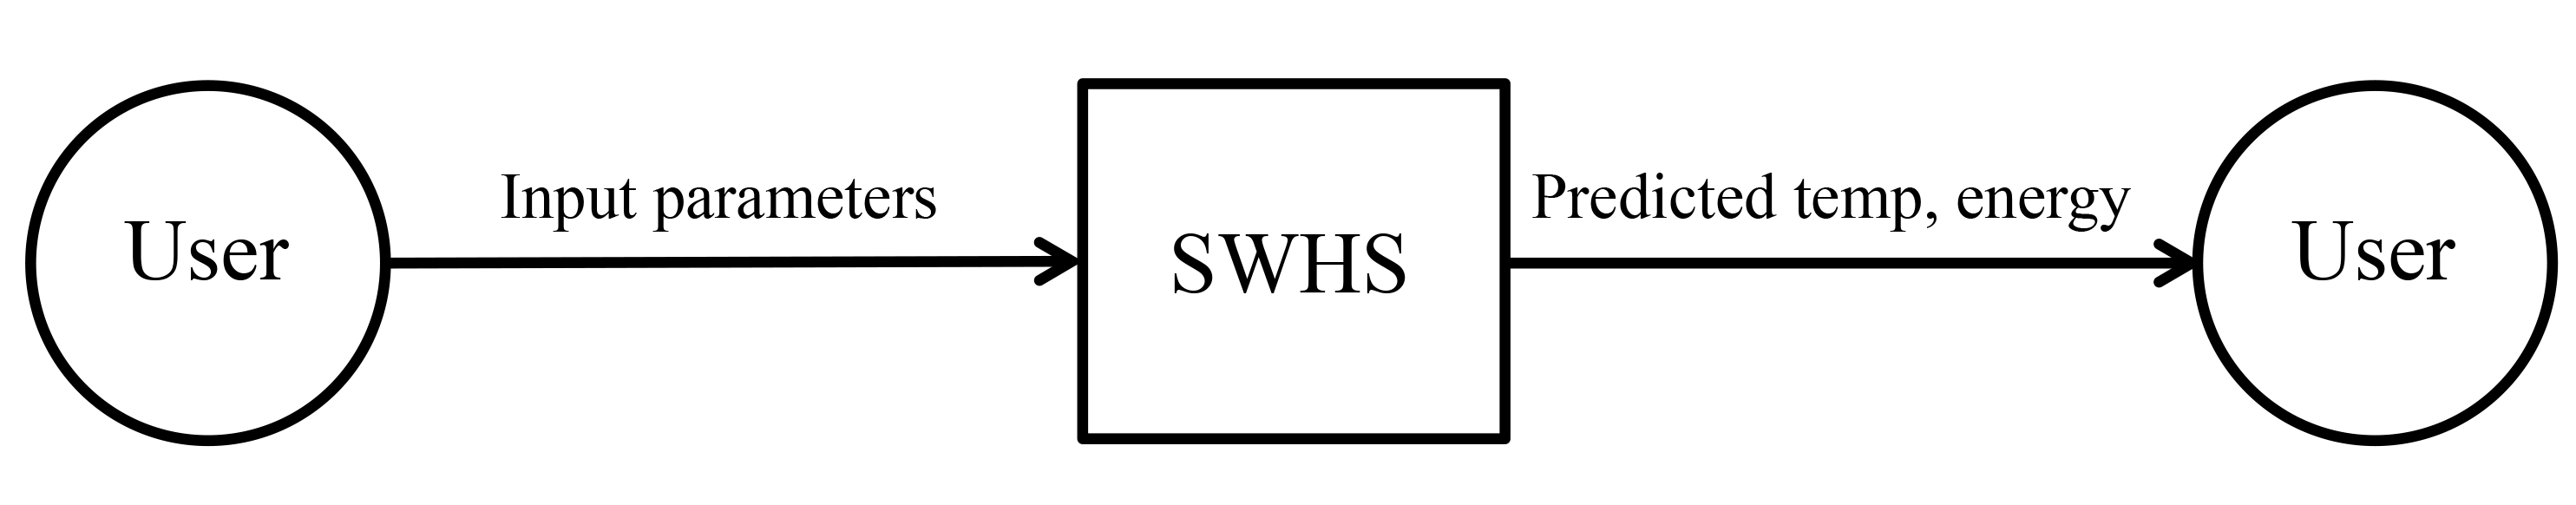
\includegraphics[width=\textwidth]{../../../../datafiles/swhs/SystemContextFigure.png}
\caption{\hyperref[Figure:SysCon]{Fig:SysCon}: System Context}
\label{Figure:SysCon}
\end{center}
\end{figure}
SWHS is mostly self-contained. The only external interaction is through the user interface. The responsibilities of the user and the system are as follows:

\begin{itemize}
\item{User Responsibilities:}
\begin{itemize}
\item{Provide the input data to the system, ensuring no errors in the data entry}
\item{Take care that consistent units are used for input variables}
\end{itemize}
\item{SWHS Responsibilities:}
\begin{itemize}
\item{Detect data type mismatch, such as a string of characters instead of a floating point number}
\item{Determine if the inputs satisfy the required physical and software constraints}
\item{Calculate the required outputs}
\end{itemize}
\end{itemize}
\subsection{User Characteristics}
\label{Sec:UserChars}
The end user of SWHS should have an understanding of undergraduate Level 1 Calculus and Physics.

\subsection{System Constraints}
\label{Sec:SysConstraints}
There are no system constraints.

\section{Specific System Description}
\label{Sec:SpecSystDesc}
This section first presents the problem description, which gives a high-level view of the problem to be solved. This is followed by the solution characteristics specification, which presents the assumptions, theories, and definitions that are used.

\subsection{Problem Description}
\label{Sec:ProbDesc}
A system is needed to investigate the effect of employing PCM within a solar water heating tank.

\subsubsection{Terminology and Definitions}
\label{Sec:TermDefs}
This subsection provides a list of terms that are used in the subsequent sections and their meaning, with the purpose of reducing ambiguity and making it easier to correctly understand the requirements.

\begin{itemize}
\item{Heat flux: The rate of thermal energy transfer through a given surface per unit time.}
\item{Phase change material: A substance that uses phase changes (such as melting) to absorb or release large amounts of heat at a constant temperature.}
\item{Specific heat capacity: The amount of energy required to raise the temperature of the unit mass of a given substance by a given amount.}
\item{Thermal conduction: The transfer of heat energy through a substance.}
\item{Transient: Changing with time.}
\end{itemize}
\subsubsection{Physical System Description}
\label{Sec:PhysSyst}
The physical system of SWHS, as shown in \hyperref[Figure:Tank]{Fig:Tank}, includes the following elements:

\begin{itemize}
\item[PS1:]{Tank containing water.}
\item[PS2:]{Heating coil at bottom of tank. (${q_{\text{C}}}$ represents the heat flux into the water from the coil.)}
\item[PS3:]{PCM suspended in tank. (${q_{\text{P}}}$ represents the heat flux into the PCM from water.)}
\end{itemize}
\begin{figure}
\begin{center}
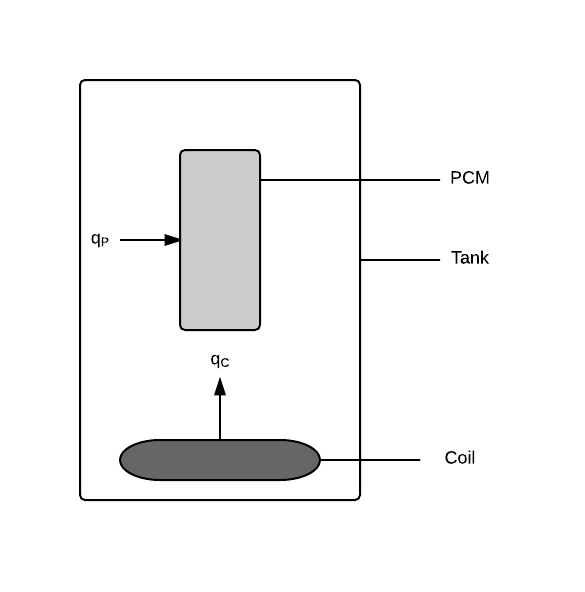
\includegraphics[width=\textwidth]{../../../../datafiles/swhs/Tank.png}
\caption{Solar water heating tank, with heat flux into the water from the coil of ${q_{\text{C}}}$ and heat flux into the PCM from water of ${q_{\text{P}}}$}
\label{Figure:Tank}
\end{center}
\end{figure}
\subsubsection{Goal Statements}
\label{Sec:GoalStmt}
Given the temperature of the heating coil, the initial conditions for the temperature of the water and the temperature of the phase change material, and the material properties, the goal statements are:

\begin{itemize}
\item[Predict-Water-Temperature:\phantomsection\label{waterTempGS}]{Predict the temperature of the water over time.}
\item[Predict-PCM-Temperature:\phantomsection\label{pcmTempGS}]{Predict the temperature of the phase change material over time.}
\item[Predict-Water-Energy:\phantomsection\label{waterEnergyGS}]{Predict the change in heat energy in the water over time.}
\item[Predict-PCM-Energy:\phantomsection\label{pcmEnergyGS}]{Predict the change in heat energy in the PCM over time.}
\end{itemize}
\subsection{Solution Characteristics Specification}
\label{Sec:SolCharSpec}
The instance models that govern SWHS are presented in the \hyperref[Sec:IMs]{Instance Model Section}. The information to understand the meaning of the instance models and their derivation is also presented, so that the instance models can be verified.

\subsubsection{Assumptions}
\label{Sec:Assumps}
This section simplifies the original problem and helps in developing the theoretical models by filling in the missing information for the physical system. The assumptions refine the scope by providing more detail.

\begin{itemize}
\item[Thermal-Energy-Only:\phantomsection\label{assumpTEO}]{The only form of energy that is relevant for this problem is thermal energy. All other forms of energy, such as mechanical energy, are assumed to be negligible. (RefBy: \hyperref[TM:consThermE]{TM:consThermE}.)}
\item[Heat-Transfer-Coeffs-Constant:\phantomsection\label{assumpHTCC}]{All heat transfer coefficients are constant over time. (RefBy: \hyperref[TM:nwtnCooling]{TM:nwtnCooling}.)}
\item[Constant-Water-Temp-Across-Tank:\phantomsection\label{assumpCWTAT}]{The water in the tank is fully mixed, so the temperature of the water is the same throughout the entire tank. (RefBy: \hyperref[GD:rocTempSimp]{GD:rocTempSimp}, \hyperref[IM:eBalanceOnWtr]{IM:eBalanceOnWtr}, and \hyperref[IM:eBalanceOnPCM]{IM:eBalanceOnPCM}.)}
\item[Temp-PCM-Constant-Across-Volume:\phantomsection\label{assumpTPCAV}]{The temperature of the phase change material is the same throughout the volume of PCM. (RefBy: \hyperref[GD:rocTempSimp]{GD:rocTempSimp}, \hyperref[likeChgUTP]{LC:Uniform-Temperature-PCM}, \hyperref[IM:eBalanceOnWtr]{IM:eBalanceOnWtr}, and \hyperref[IM:eBalanceOnPCM]{IM:eBalanceOnPCM}.)}
\item[Density-Water-PCM-Constant-over-Volume:\phantomsection\label{assumpDWPCoV}]{The density of water and density of PCM have no spatial variation; that is, they are each constant over their entire volume. (RefBy: \hyperref[GD:rocTempSimp]{GD:rocTempSimp}.)}
\item[Specific-Heat-Energy-Constant-over-Volume:\phantomsection\label{assumpSHECov}]{The specific heat capacity of water, specific heat capacity of PCM as a solid, and specific heat capacity of PCM as a liquid have no spatial variation; that is, they are each constant over their entire volume. (RefBy: \hyperref[GD:rocTempSimp]{GD:rocTempSimp}.)}
\item[Newton-Law-Convective-Cooling-Coil-Water:\phantomsection\label{assumpLCCCW}]{Newton's law of convective cooling applies between the heating coil and the water. (RefBy: \hyperref[GD:htFluxWaterFromCoil]{GD:htFluxWaterFromCoil}.)}
\item[Temp-Heating-Coil-Constant-over-Time:\phantomsection\label{assumpTHCCoT}]{The temperature of the heating coil is constant over time. (RefBy: \hyperref[likeChgTCVOD]{LC:Temperature-Coil-Variable-Over-Day} and \hyperref[GD:htFluxWaterFromCoil]{GD:htFluxWaterFromCoil}.)}
\item[Temp-Heating-Coil-Constant-over-Length:\phantomsection\label{assumpTHCCoL}]{The temperature of the heating coil does not vary along its length. (RefBy: \hyperref[likeChgTCVOL]{LC:Temperature-Coil-Variable-Over-Length} and \hyperref[IM:eBalanceOnWtr]{IM:eBalanceOnWtr}.)}
\item[Law-Convective-Cooling-Water-PCM:\phantomsection\label{assumpLCCWP}]{Newton's law of convective cooling applies between the water and the PCM. (RefBy: \hyperref[GD:htFluxPCMFromWater]{GD:htFluxPCMFromWater}.)}
\item[Charging-Tank-No-Temp-Discharge:\phantomsection\label{assumpCTNOD}]{The model only accounts for charging of the tank, not discharging. The temperature of the water and temperature of the phase change material can only increase, or remain constant; they do not decrease. This implies that the initial temperature \hyperref[assumpSITWP]{A:Same-Initial-Temp-Water-PCM} is less than (or equal) to the temperature of the heating coil. (RefBy: \hyperref[likeChgDT]{LC:Discharging-Tank} and \hyperref[IM:eBalanceOnWtr]{IM:eBalanceOnWtr}.)}
\item[Same-Initial-Temp-Water-PCM:\phantomsection\label{assumpSITWP}]{The initial temperature of the water and the PCM is the same. (RefBy: \hyperref[likeChgDITPW]{LC:Different-Initial-Temps-PCM-Water}, \hyperref[IM:eBalanceOnWtr]{IM:eBalanceOnWtr}, \hyperref[IM:eBalanceOnPCM]{IM:eBalanceOnPCM}, and \hyperref[assumpCTNOD]{A:Charging-Tank-No-Temp-Discharge}.)}
\item[PCM-Initially-Solid:\phantomsection\label{assumpPIS}]{The simulation will start with the PCM in a solid state. (RefBy: \hyperref[IM:heatEInPCM]{IM:heatEInPCM} and \hyperref[IM:eBalanceOnPCM]{IM:eBalanceOnPCM}.)}
\item[Water-Always-Liquid:\phantomsection\label{assumpWAL}]{The operating temperature range of the system is such that the water is always in liquid state. That is, the temperature will not drop below the melting point temperature of water, or rise above its boiling point temperature. (RefBy: \hyperref[unlikeChgWPFS]{UC:Water-PCM-Fixed-States}, \hyperref[IM:heatEInWtr]{IM:heatEInWtr}, and \hyperref[IM:eBalanceOnWtr]{IM:eBalanceOnWtr}.)}
\item[Perfect-Insulation-Tank:\phantomsection\label{assumpPIT}]{The tank is perfectly insulated so that there is no heat loss from the tank. (RefBy: \hyperref[likeChgTLH]{LC:Tank-Lose-Heat} and \hyperref[IM:eBalanceOnWtr]{IM:eBalanceOnWtr}.)}
\item[No-Internal-Heat-Generation-By-Water-PCM:\phantomsection\label{assumpNIHGBWP}]{No internal heat is generated by either the water or the PCM; therefore, the volumetric heat generation per unit volume is zero. (RefBy: \hyperref[unlikeChgNIHG]{UC:No-Internal-Heat-Generation}, \hyperref[IM:eBalanceOnWtr]{IM:eBalanceOnWtr}, and \hyperref[IM:eBalanceOnPCM]{IM:eBalanceOnPCM}.)}
\item[Volume-Change-Melting-PCM-Negligible:\phantomsection\label{assumpVCMPN}]{The volume change of the PCM due to melting is negligible. (RefBy: \hyperref[IM:eBalanceOnPCM]{IM:eBalanceOnPCM}.)}
\item[No-Gaseous-State-PCM:\phantomsection\label{assumpNGSP}]{The PCM is either in a liquid state or a solid state but not a gaseous state. (RefBy: \hyperref[unlikeChgWPFS]{UC:Water-PCM-Fixed-States}, \hyperref[unlikeChgNGS]{UC:No-Gaseous-State}, \hyperref[IM:heatEInPCM]{IM:heatEInPCM}, and \hyperref[IM:eBalanceOnPCM]{IM:eBalanceOnPCM}.)}
\item[Atmospheric-Pressure-Tank:\phantomsection\label{assumpAPT}]{The pressure in the tank is atmospheric, so the melting point temperature and boiling point temperature are 0${{}^{\circ}\text{C}}$ and 100${{}^{\circ}\text{C}}$, respectively. (RefBy: \hyperref[IM:heatEInWtr]{IM:heatEInWtr} and \hyperref[IM:eBalanceOnWtr]{IM:eBalanceOnWtr}.)}
\item[Volume-Coil-Negligible:\phantomsection\label{assumpVCN}]{When considering the volume of water in the tank, the volume of the heating coil is assumed to be negligible. (RefBy: \hyperref[DD:waterVolume.pcm]{DD:waterVolume\_pcm}.)}
\end{itemize}
\subsubsection{Theoretical Models}
\label{Sec:TMs}
This section focuses on the general equations and laws that SWHS is based on.

\vspace{\baselineskip}
\noindent
\begin{minipage}{\textwidth}
\begin{tabular}{>{\raggedright}p{0.13\textwidth}>{\raggedright\arraybackslash}p{0.82\textwidth}}
\toprule \textbf{Refname} & \textbf{TM:consThermE}
\phantomsection 
\label{TM:consThermE}
\\ \midrule \\
Label & Conservation of thermal energy
        
\\ \midrule \\
Equation & \begin{displaymath}
           -∇\cdot{}\symbf{q}+g=ρ C \frac{\,\partial{}T}{\,\partial{}t}
           \end{displaymath}
\\ \midrule \\
Description & \begin{symbDescription}
              \item{$∇$ is the gradient (Unitless)}
              \item{$\symbf{q}$ is the thermal flux vector ($\frac{\text{W}}{\text{m}^{2}}$)}
              \item{$g$ is the volumetric heat generation per unit volume ($\frac{\text{W}}{\text{m}^{3}}$)}
              \item{$ρ$ is the density ($\frac{\text{kg}}{\text{m}^{3}}$)}
              \item{$C$ is the specific heat capacity ($\frac{\text{J}}{\text{kg}{}^{\circ}\text{C}}$)}
              \item{$t$ is the time (${\text{s}}$)}
              \item{$T$ is the temperature (${{}^{\circ}\text{C}}$)}
              \end{symbDescription}
\\ \midrule \\
Notes & The above equation gives the law of conservation of energy for transient heat transfer in a given material.
        
        For this equation to apply, other forms of energy, such as mechanical energy, are assumed to be negligible in the system (\hyperref[assumpTEO]{A:Thermal-Energy-Only}).
        
\\ \midrule \\
Source & \hyperref{http://www.efunda.com/formulae/heat_transfer/conduction/overview_cond.cfm}{}{}{Fourier Law of Heat Conduction and Heat Equation}
         
\\ \midrule \\
RefBy & \hyperref[GD:rocTempSimp]{GD:rocTempSimp}
        
\\ \bottomrule
\end{tabular}
\end{minipage}
\vspace{\baselineskip}
\noindent
\begin{minipage}{\textwidth}
\begin{tabular}{>{\raggedright}p{0.13\textwidth}>{\raggedright\arraybackslash}p{0.82\textwidth}}
\toprule \textbf{Refname} & \textbf{TM:sensHtE}
\phantomsection 
\label{TM:sensHtE}
\\ \midrule \\
Label & Sensible heat energy
        
\\ \midrule \\
Equation & \begin{displaymath}
           E=\begin{cases}
             {C^{\text{S}}} m ΔT, & T\lt{}{T_{\text{melt}}}\\
             {C^{\text{L}}} m ΔT, & {T_{\text{melt}}}\lt{}T\lt{}{T_{\text{boil}}}\\
             {C^{\text{V}}} m ΔT, & {T_{\text{boil}}}\lt{}T
             \end{cases}
           \end{displaymath}
\\ \midrule \\
Description & \begin{symbDescription}
              \item{$E$ is the sensible heat (${\text{J}}$)}
              \item{${C^{\text{S}}}$ is the specific heat capacity of a solid ($\frac{\text{J}}{\text{kg}{}^{\circ}\text{C}}$)}
              \item{$m$ is the mass (${\text{kg}}$)}
              \item{$ΔT$ is the change in temperature (${{}^{\circ}\text{C}}$)}
              \item{${C^{\text{L}}}$ is the specific heat capacity of a liquid ($\frac{\text{J}}{\text{kg}{}^{\circ}\text{C}}$)}
              \item{${C^{\text{V}}}$ is the specific heat capacity of a vapour ($\frac{\text{J}}{\text{kg}{}^{\circ}\text{C}}$)}
              \item{$T$ is the temperature (${{}^{\circ}\text{C}}$)}
              \item{${T_{\text{melt}}}$ is the melting point temperature (${{}^{\circ}\text{C}}$)}
              \item{${T_{\text{boil}}}$ is the boiling point temperature (${{}^{\circ}\text{C}}$)}
              \end{symbDescription}
\\ \midrule \\
Notes & Sensible heating occurs as long as the material does not reach a temperature where a phase change occurs. A phase change occurs if $T={T_{\text{boil}}}$ or $T={T_{\text{melt}}}$. If this is the case, refer to \hyperref[TM:latentHtE]{TM:latentHtE}.
        
\\ \midrule \\
Source & \hyperref{http://en.wikipedia.org/wiki/Sensible_heat}{}{}{Definition of Sensible Heat}
         
\\ \midrule \\
RefBy & \hyperref[IM:heatEInWtr]{IM:heatEInWtr} and \hyperref[IM:heatEInPCM]{IM:heatEInPCM}
        
\\ \bottomrule
\end{tabular}
\end{minipage}
\vspace{\baselineskip}
\noindent
\begin{minipage}{\textwidth}
\begin{tabular}{>{\raggedright}p{0.13\textwidth}>{\raggedright\arraybackslash}p{0.82\textwidth}}
\toprule \textbf{Refname} & \textbf{TM:latentHtE}
\phantomsection 
\label{TM:latentHtE}
\\ \midrule \\
Label & Latent heat energy
        
\\ \midrule \\
Equation & \begin{displaymath}
           Q\left(t\right)=\int_{0}^{t}{\frac{\,dQ\left(τ\right)}{\,dτ}}\,dτ
           \end{displaymath}
\\ \midrule \\
Description & \begin{symbDescription}
              \item{$Q$ is the latent heat (${\text{J}}$)}
              \item{$t$ is the time (${\text{s}}$)}
              \item{$τ$ is the dummy variable for integration over time (${\text{s}}$)}
              \end{symbDescription}
\\ \midrule \\
Notes & $Q$ is the change in thermal energy (latent heat energy).
        
        $Q\left(t\right)=\int_{0}^{t}{\frac{\,dQ\left(τ\right)}{\,dτ}}\,dτ$ is the rate of change of $Q$ with respect to time $τ$.
        
        $t$ is the time elapsed, as long as the phase change is not complete.
        
        The status of the phase change depends on the melt fraction (from \hyperref[DD:meltFrac]{DD:meltFrac}).
        
        Latent heating stops when all material has changed to the new phase.
        
\\ \midrule \\
Source & \hyperref{http://en.wikipedia.org/wiki/Latent_heat}{}{}{Definition of Latent Heat}
         
\\ \midrule \\
RefBy & \hyperref[TM:sensHtE]{TM:sensHtE} and \hyperref[IM:heatEInPCM]{IM:heatEInPCM}
        
\\ \bottomrule
\end{tabular}
\end{minipage}
\vspace{\baselineskip}
\noindent
\begin{minipage}{\textwidth}
\begin{tabular}{>{\raggedright}p{0.13\textwidth}>{\raggedright\arraybackslash}p{0.82\textwidth}}
\toprule \textbf{Refname} & \textbf{TM:nwtnCooling}
\phantomsection 
\label{TM:nwtnCooling}
\\ \midrule \\
Label & Newton's law of cooling
        
\\ \midrule \\
Equation & \begin{displaymath}
           q\left(t\right)=h ΔT\left(t\right)
           \end{displaymath}
\\ \midrule \\
Description & \begin{symbDescription}
              \item{$q$ is the heat flux ($\frac{\text{W}}{\text{m}^{2}}$)}
              \item{$t$ is the time (${\text{s}}$)}
              \item{$h$ is the convective heat transfer coefficient ($\frac{\text{W}}{\text{m}^{2}{}^{\circ}\text{C}}$)}
              \item{$ΔT$ is the change in temperature (${{}^{\circ}\text{C}}$)}
              \end{symbDescription}
\\ \midrule \\
Notes & Newton's law of cooling describes convective cooling from a surface. The law is stated as: the rate of heat loss from a body is proportional to the difference in temperatures between the body and its surroundings.
        
        $h$ is assumed to be independent of $T$ (from \hyperref[assumpHTCC]{A:Heat-Transfer-Coeffs-Constant}).
        
        $ΔT\left(t\right)=T\left(t\right)-{T_{\text{env}}}\left(t\right)$ is the time-dependant thermal gradient between the environment and the object.
        
\\ \midrule \\
Source & \cite[(pg. 8)]{incroperaEtAl2007}
         
\\ \midrule \\
RefBy & \hyperref[GD:htFluxPCMFromWater]{GD:htFluxPCMFromWater} and \hyperref[GD:htFluxWaterFromCoil]{GD:htFluxWaterFromCoil}
        
\\ \bottomrule
\end{tabular}
\end{minipage}
\subsubsection{General Definitions}
\label{Sec:GDs}
This section collects the laws and equations that will be used to build the instance models.

\vspace{\baselineskip}
\noindent
\begin{minipage}{\textwidth}
\begin{tabular}{>{\raggedright}p{0.13\textwidth}>{\raggedright\arraybackslash}p{0.82\textwidth}}
\toprule \textbf{Refname} & \textbf{GD:rocTempSimp}
\phantomsection 
\label{GD:rocTempSimp}
\\ \midrule \\
Label & Simplified rate of change of temperature
        
\\ \midrule \\
Equation & \begin{displaymath}
           m C \frac{\,dT}{\,dt}={q_{\text{in}}} {A_{\text{in}}}-{q_{\text{out}}} {A_{\text{out}}}+g V
           \end{displaymath}
\\ \midrule \\
Description & \begin{symbDescription}
              \item{$m$ is the mass (${\text{kg}}$)}
              \item{$C$ is the specific heat capacity ($\frac{\text{J}}{\text{kg}{}^{\circ}\text{C}}$)}
              \item{$t$ is the time (${\text{s}}$)}
              \item{$T$ is the temperature (${{}^{\circ}\text{C}}$)}
              \item{${q_{\text{in}}}$ is the heat flux input ($\frac{\text{W}}{\text{m}^{2}}$)}
              \item{${A_{\text{in}}}$ is the surface area over which heat is transferred in (${\text{m}^{2}}$)}
              \item{${q_{\text{out}}}$ is the heat flux output ($\frac{\text{W}}{\text{m}^{2}}$)}
              \item{${A_{\text{out}}}$ is the surface area over which heat is transferred out (${\text{m}^{2}}$)}
              \item{$g$ is the volumetric heat generation per unit volume ($\frac{\text{W}}{\text{m}^{3}}$)}
              \item{$V$ is the volume (${\text{m}^{3}}$)}
              \end{symbDescription}
\\ \midrule \\
Source & --
         
\\ \midrule \\
RefBy & \hyperref[GD:rocTempSimp]{GD:rocTempSimp}, \hyperref[IM:eBalanceOnWtr]{IM:eBalanceOnWtr}, and \hyperref[IM:eBalanceOnPCM]{IM:eBalanceOnPCM}
        
\\ \bottomrule
\end{tabular}
\end{minipage}
\paragraph{Detailed derivation of simplified rate of change of temperature:}
\label{GD:rocTempSimpDeriv}
Integrating \hyperref[TM:consThermE]{TM:consThermE} over a volume ($V$), we have:

\begin{displaymath}
-\int_{V}{∇\cdot{}\symbf{q}}\,dV+\int_{V}{g}\,dV=\int_{V}{ρ C \frac{\,\partial{}T}{\,\partial{}t}}\,dV
\end{displaymath}
Applying Gauss's Divergence Theorem to the first term over the surface $S$ of the volume, with $\symbf{q}$ as the thermal flux vector for the surface and $\symbf{\hat{n}}$ as a unit outward normal vector for a surface:

\begin{displaymath}
-\int_{S}{\symbf{q}\cdot{}\symbf{\hat{n}}}\,dS+\int_{V}{g}\,dV=\int_{V}{ρ C \frac{\,\partial{}T}{\,\partial{}t}}\,dV
\end{displaymath}
We consider an arbitrary volume. The volumetric heat generation per unit volume is assumed constant. Then Equation (1) can be written as:

\begin{displaymath}
{q_{\text{in}}} {A_{\text{in}}}-{q_{\text{out}}} {A_{\text{out}}}+g V=\int_{V}{ρ C \frac{\,\partial{}T}{\,\partial{}t}}\,dV
\end{displaymath}
Where ${q_{\text{in}}}$, ${q_{\text{out}}}$, ${A_{\text{in}}}$, and ${A_{\text{out}}}$ are explained in \hyperref[GD:rocTempSimp]{GD:rocTempSimp}. The integral over the surface could be simplified because the thermal flux is assumed constant over ${A_{\text{in}}}$ and ${A_{\text{out}}}$ and $0$ on all other surfaces. Outward flux is considered positive. Assuming $ρ$, $C$, and $T$ are constant over the volume, which is true in our case by \hyperref[assumpCWTAT]{A:Constant-Water-Temp-Across-Tank}, \hyperref[assumpTPCAV]{A:Temp-PCM-Constant-Across-Volume}, \hyperref[assumpDWPCoV]{A:Density-Water-PCM-Constant-over-Volume}, and \hyperref[assumpSHECov]{A:Specific-Heat-Energy-Constant-over-Volume}, we have:

\begin{displaymath}
ρ C V \frac{\,dT}{\,dt}={q_{\text{in}}} {A_{\text{in}}}-{q_{\text{out}}} {A_{\text{out}}}+g V
\end{displaymath}
Using the fact that $ρ$=$m$/$V$, Equation (2) can be written as:

\begin{displaymath}
m C \frac{\,dT}{\,dt}={q_{\text{in}}} {A_{\text{in}}}-{q_{\text{out}}} {A_{\text{out}}}+g V
\end{displaymath}
\vspace{\baselineskip}
\noindent
\begin{minipage}{\textwidth}
\begin{tabular}{>{\raggedright}p{0.13\textwidth}>{\raggedright\arraybackslash}p{0.82\textwidth}}
\toprule \textbf{Refname} & \textbf{GD:htFluxWaterFromCoil}
\phantomsection 
\label{GD:htFluxWaterFromCoil}
\\ \midrule \\
Label & Heat flux into the water from the coil
        
\\ \midrule \\
Units & $\frac{\text{W}}{\text{m}^{2}}$
        
\\ \midrule \\
Equation & \begin{displaymath}
           {q_{\text{C}}}={h_{\text{C}}} \left({T_{\text{C}}}-{T_{\text{W}}}\left(t\right)\right)
           \end{displaymath}
\\ \midrule \\
Description & \begin{symbDescription}
              \item{${q_{\text{C}}}$ is the heat flux into the water from the coil ($\frac{\text{W}}{\text{m}^{2}}$)}
              \item{${h_{\text{C}}}$ is the convective heat transfer coefficient between coil and water ($\frac{\text{W}}{\text{m}^{2}{}^{\circ}\text{C}}$)}
              \item{${T_{\text{C}}}$ is the temperature of the heating coil (${{}^{\circ}\text{C}}$)}
              \item{${T_{\text{W}}}$ is the temperature of the water (${{}^{\circ}\text{C}}$)}
              \item{$t$ is the time (${\text{s}}$)}
              \end{symbDescription}
\\ \midrule \\
Notes & ${q_{\text{C}}}$ is found by assuming that Newton's law of cooling applies (\hyperref[assumpLCCCW]{A:Newton-Law-Convective-Cooling-Coil-Water}). This law (defined in \hyperref[TM:nwtnCooling]{TM:nwtnCooling}) is used on the surface of the heating coil.
        
        \hyperref[assumpTHCCoT]{A:Temp-Heating-Coil-Constant-over-Time}
        
\\ \midrule \\
Source & \cite{koothoor2013}
         
\\ \midrule \\
RefBy & \hyperref[IM:eBalanceOnWtr]{IM:eBalanceOnWtr}
        
\\ \bottomrule
\end{tabular}
\end{minipage}

\vspace{\baselineskip}
\noindent
\begin{minipage}{\textwidth}
\begin{tabular}{>{\raggedright}p{0.13\textwidth}>{\raggedright\arraybackslash}p{0.82\textwidth}}
\toprule \textbf{Refname} & \textbf{GD:htFluxPCMFromWater}
\phantomsection 
\label{GD:htFluxPCMFromWater}
\\ \midrule \\
Label & Heat flux into the PCM from water
        
\\ \midrule \\
Units & $\frac{\text{W}}{\text{m}^{2}}$
        
\\ \midrule \\
Equation & \begin{displaymath}
           {q_{\text{P}}}={h_{\text{P}}} \left({T_{\text{W}}}\left(t\right)-{T_{\text{P}}}\left(t\right)\right)
           \end{displaymath}
\\ \midrule \\
Description & \begin{symbDescription}
              \item{${q_{\text{P}}}$ is the heat flux into the PCM from water ($\frac{\text{W}}{\text{m}^{2}}$)}
              \item{${h_{\text{P}}}$ is the convective heat transfer coefficient between PCM and water ($\frac{\text{W}}{\text{m}^{2}{}^{\circ}\text{C}}$)}
              \item{${T_{\text{W}}}$ is the temperature of the water (${{}^{\circ}\text{C}}$)}
              \item{$t$ is the time (${\text{s}}$)}
              \item{${T_{\text{P}}}$ is the temperature of the phase change material (${{}^{\circ}\text{C}}$)}
              \end{symbDescription}
\\ \midrule \\
Notes & ${q_{\text{P}}}$ is found by assuming that Newton's law of cooling applies (\hyperref[assumpLCCWP]{A:Law-Convective-Cooling-Water-PCM}). This law (defined in \hyperref[TM:nwtnCooling]{TM:nwtnCooling}) is used on the surface of the phase change material.
        
\\ \midrule \\
Source & \cite{koothoor2013}
         
\\ \midrule \\
RefBy & \hyperref[IM:eBalanceOnWtr]{IM:eBalanceOnWtr} and \hyperref[IM:eBalanceOnPCM]{IM:eBalanceOnPCM}
        
\\ \bottomrule
\end{tabular}
\end{minipage}

\subsubsection{Data Definitions}
\label{Sec:DDs}
This section collects and defines all the data needed to build the instance models.

\vspace{\baselineskip}
\noindent
\begin{minipage}{\textwidth}
\begin{tabular}{>{\raggedright}p{0.13\textwidth}>{\raggedright\arraybackslash}p{0.82\textwidth}}
\toprule \textbf{Refname} & \textbf{DD:waterMass}
\phantomsection 
\label{DD:waterMass}
\\ \midrule \\
Label & Mass of water
        
\\ \midrule \\
Symbol & ${m_{\text{W}}}$
         
\\ \midrule \\
Units & ${\text{kg}}$
        
\\ \midrule \\
Equation & \begin{displaymath}
           {m_{\text{W}}}={V_{\text{W}}} {ρ_{\text{W}}}
           \end{displaymath}
\\ \midrule \\
Description & \begin{symbDescription}
              \item{${m_{\text{W}}}$ is the mass of water (${\text{kg}}$)}
              \item{${V_{\text{W}}}$ is the volume of water (${\text{m}^{3}}$)}
              \item{${ρ_{\text{W}}}$ is the density of water ($\frac{\text{kg}}{\text{m}^{3}}$)}
              \end{symbDescription}
\\ \midrule \\
Source & --
         
\\ \midrule \\
RefBy & \hyperref[findMass]{FR:Find-Mass}
        
\\ \bottomrule
\end{tabular}
\end{minipage}

\vspace{\baselineskip}
\noindent
\begin{minipage}{\textwidth}
\begin{tabular}{>{\raggedright}p{0.13\textwidth}>{\raggedright\arraybackslash}p{0.82\textwidth}}
\toprule \textbf{Refname} & \textbf{DD:waterVolume.pcm}
\phantomsection 
\label{DD:waterVolume.pcm}
\\ \midrule \\
Label & Volume of water
        
\\ \midrule \\
Symbol & ${V_{\text{W}}}$
         
\\ \midrule \\
Units & ${\text{m}^{3}}$
        
\\ \midrule \\
Equation & \begin{displaymath}
           {V_{\text{W}}}={V_{\text{tank}}}-{V_{\text{P}}}
           \end{displaymath}
\\ \midrule \\
Description & \begin{symbDescription}
              \item{${V_{\text{W}}}$ is the volume of water (${\text{m}^{3}}$)}
              \item{${V_{\text{tank}}}$ is the volume of the cylindrical tank (${\text{m}^{3}}$)}
              \item{${V_{\text{P}}}$ is the volume of PCM (${\text{m}^{3}}$)}
              \end{symbDescription}
\\ \midrule \\
Notes & Based on \hyperref[assumpVCN]{A:Volume-Coil-Negligible}. ${V_{\text{tank}}}$ is defined in \hyperref[DD:tankVolume]{DD:tankVolume}.
        
\\ \midrule \\
Source & --
         
\\ \midrule \\
RefBy & \hyperref[findMass]{FR:Find-Mass}
        
\\ \bottomrule
\end{tabular}
\end{minipage}

\vspace{\baselineskip}
\noindent
\begin{minipage}{\textwidth}
\begin{tabular}{>{\raggedright}p{0.13\textwidth}>{\raggedright\arraybackslash}p{0.82\textwidth}}
\toprule \textbf{Refname} & \textbf{DD:tankVolume}
\phantomsection 
\label{DD:tankVolume}
\\ \midrule \\
Label & Volume of the cylindrical tank
        
\\ \midrule \\
Symbol & ${V_{\text{tank}}}$
         
\\ \midrule \\
Units & ${\text{m}^{3}}$
        
\\ \midrule \\
Equation & \begin{displaymath}
           {V_{\text{tank}}}=π \left(\frac{D}{2}\right)^{2} L
           \end{displaymath}
\\ \midrule \\
Description & \begin{symbDescription}
              \item{${V_{\text{tank}}}$ is the volume of the cylindrical tank (${\text{m}^{3}}$)}
              \item{$π$ is the ratio of circumference to diameter for any circle (Unitless)}
              \item{$D$ is the diameter of tank (${\text{m}}$)}
              \item{$L$ is the length of tank (${\text{m}}$)}
              \end{symbDescription}
\\ \midrule \\
Source & --
         
\\ \midrule \\
RefBy & \hyperref[DD:waterVolume.pcm]{DD:waterVolume\_pcm} and \hyperref[findMass]{FR:Find-Mass}
        
\\ \bottomrule
\end{tabular}
\end{minipage}

\vspace{\baselineskip}
\noindent
\begin{minipage}{\textwidth}
\begin{tabular}{>{\raggedright}p{0.13\textwidth}>{\raggedright\arraybackslash}p{0.82\textwidth}}
\toprule \textbf{Refname} & \textbf{DD:balanceDecayRate}
\phantomsection 
\label{DD:balanceDecayRate}
\\ \midrule \\
Label & ODE parameter for water related to decay time
        
\\ \midrule \\
Symbol & ${τ_{\text{W}}}$
         
\\ \midrule \\
Units & ${\text{s}}$
        
\\ \midrule \\
Equation & \begin{displaymath}
           {τ_{\text{W}}}=\frac{{m_{\text{W}}} {C_{\text{W}}}}{{h_{\text{C}}} {A_{\text{C}}}}
           \end{displaymath}
\\ \midrule \\
Description & \begin{symbDescription}
              \item{${τ_{\text{W}}}$ is the ODE parameter for water related to decay time (${\text{s}}$)}
              \item{${m_{\text{W}}}$ is the mass of water (${\text{kg}}$)}
              \item{${C_{\text{W}}}$ is the specific heat capacity of water ($\frac{\text{J}}{\text{kg}{}^{\circ}\text{C}}$)}
              \item{${h_{\text{C}}}$ is the convective heat transfer coefficient between coil and water ($\frac{\text{W}}{\text{m}^{2}{}^{\circ}\text{C}}$)}
              \item{${A_{\text{C}}}$ is the heating coil surface area (${\text{m}^{2}}$)}
              \end{symbDescription}
\\ \midrule \\
Source & \cite{koothoor2013}
         
\\ \midrule \\
RefBy & \hyperref[outputInputDerivVals]{FR:Output-Input-Derived-Values} and \hyperref[IM:eBalanceOnWtr]{IM:eBalanceOnWtr}
        
\\ \bottomrule
\end{tabular}
\end{minipage}

\vspace{\baselineskip}
\noindent
\begin{minipage}{\textwidth}
\begin{tabular}{>{\raggedright}p{0.13\textwidth}>{\raggedright\arraybackslash}p{0.82\textwidth}}
\toprule \textbf{Refname} & \textbf{DD:balanceDecayTime}
\phantomsection 
\label{DD:balanceDecayTime}
\\ \midrule \\
Label & ODE parameter related to decay rate
        
\\ \midrule \\
Symbol & $η$
         
\\ \midrule \\
Units & Unitless
        
\\ \midrule \\
Equation & \begin{displaymath}
           η=\frac{{h_{\text{P}}} {A_{\text{P}}}}{{h_{\text{C}}} {A_{\text{C}}}}
           \end{displaymath}
\\ \midrule \\
Description & \begin{symbDescription}
              \item{$η$ is the ODE parameter related to decay rate (Unitless)}
              \item{${h_{\text{P}}}$ is the convective heat transfer coefficient between PCM and water ($\frac{\text{W}}{\text{m}^{2}{}^{\circ}\text{C}}$)}
              \item{${A_{\text{P}}}$ is the phase change material surface area (${\text{m}^{2}}$)}
              \item{${h_{\text{C}}}$ is the convective heat transfer coefficient between coil and water ($\frac{\text{W}}{\text{m}^{2}{}^{\circ}\text{C}}$)}
              \item{${A_{\text{C}}}$ is the heating coil surface area (${\text{m}^{2}}$)}
              \end{symbDescription}
\\ \midrule \\
Source & \cite{koothoor2013}
         
\\ \midrule \\
RefBy & \hyperref[outputInputDerivVals]{FR:Output-Input-Derived-Values} and \hyperref[IM:eBalanceOnWtr]{IM:eBalanceOnWtr}
        
\\ \bottomrule
\end{tabular}
\end{minipage}

\vspace{\baselineskip}
\noindent
\begin{minipage}{\textwidth}
\begin{tabular}{>{\raggedright}p{0.13\textwidth}>{\raggedright\arraybackslash}p{0.82\textwidth}}
\toprule \textbf{Refname} & \textbf{DD:balanceSolidPCM}
\phantomsection 
\label{DD:balanceSolidPCM}
\\ \midrule \\
Label & ODE parameter for solid PCM
        
\\ \midrule \\
Symbol & ${{τ_{\text{P}}}^{\text{S}}}$
         
\\ \midrule \\
Units & ${\text{s}}$
        
\\ \midrule \\
Equation & \begin{displaymath}
           {{τ_{\text{P}}}^{\text{S}}}=\frac{{m_{\text{P}}} {{C_{\text{P}}}^{\text{S}}}}{{h_{\text{P}}} {A_{\text{P}}}}
           \end{displaymath}
\\ \midrule \\
Description & \begin{symbDescription}
              \item{${{τ_{\text{P}}}^{\text{S}}}$ is the ODE parameter for solid PCM (${\text{s}}$)}
              \item{${m_{\text{P}}}$ is the mass of phase change material (${\text{kg}}$)}
              \item{${{C_{\text{P}}}^{\text{S}}}$ is the specific heat capacity of PCM as a solid ($\frac{\text{J}}{\text{kg}{}^{\circ}\text{C}}$)}
              \item{${h_{\text{P}}}$ is the convective heat transfer coefficient between PCM and water ($\frac{\text{W}}{\text{m}^{2}{}^{\circ}\text{C}}$)}
              \item{${A_{\text{P}}}$ is the phase change material surface area (${\text{m}^{2}}$)}
              \end{symbDescription}
\\ \midrule \\
Source & \cite{lightstone2012}
         
\\ \midrule \\
RefBy & \hyperref[outputInputDerivVals]{FR:Output-Input-Derived-Values} and \hyperref[IM:eBalanceOnPCM]{IM:eBalanceOnPCM}
        
\\ \bottomrule
\end{tabular}
\end{minipage}

\vspace{\baselineskip}
\noindent
\begin{minipage}{\textwidth}
\begin{tabular}{>{\raggedright}p{0.13\textwidth}>{\raggedright\arraybackslash}p{0.82\textwidth}}
\toprule \textbf{Refname} & \textbf{DD:balanceLiquidPCM}
\phantomsection 
\label{DD:balanceLiquidPCM}
\\ \midrule \\
Label & ODE parameter for liquid PCM
        
\\ \midrule \\
Symbol & ${{τ_{\text{P}}}^{\text{L}}}$
         
\\ \midrule \\
Units & ${\text{s}}$
        
\\ \midrule \\
Equation & \begin{displaymath}
           {{τ_{\text{P}}}^{\text{L}}}=\frac{{m_{\text{P}}} {{C_{\text{P}}}^{\text{L}}}}{{h_{\text{P}}} {A_{\text{P}}}}
           \end{displaymath}
\\ \midrule \\
Description & \begin{symbDescription}
              \item{${{τ_{\text{P}}}^{\text{L}}}$ is the ODE parameter for liquid PCM (${\text{s}}$)}
              \item{${m_{\text{P}}}$ is the mass of phase change material (${\text{kg}}$)}
              \item{${{C_{\text{P}}}^{\text{L}}}$ is the specific heat capacity of PCM as a liquid ($\frac{\text{J}}{\text{kg}{}^{\circ}\text{C}}$)}
              \item{${h_{\text{P}}}$ is the convective heat transfer coefficient between PCM and water ($\frac{\text{W}}{\text{m}^{2}{}^{\circ}\text{C}}$)}
              \item{${A_{\text{P}}}$ is the phase change material surface area (${\text{m}^{2}}$)}
              \end{symbDescription}
\\ \midrule \\
Source & \cite{lightstone2012}
         
\\ \midrule \\
RefBy & \hyperref[outputInputDerivVals]{FR:Output-Input-Derived-Values} and \hyperref[IM:eBalanceOnPCM]{IM:eBalanceOnPCM}
        
\\ \bottomrule
\end{tabular}
\end{minipage}

\vspace{\baselineskip}
\noindent
\begin{minipage}{\textwidth}
\begin{tabular}{>{\raggedright}p{0.13\textwidth}>{\raggedright\arraybackslash}p{0.82\textwidth}}
\toprule \textbf{Refname} & \textbf{DD:htFusion}
\phantomsection 
\label{DD:htFusion}
\\ \midrule \\
Label & Specific latent heat of fusion
        
\\ \midrule \\
Symbol & ${H_{\text{f}}}$
         
\\ \midrule \\
Units & $\frac{\text{J}}{\text{kg}}$
        
\\ \midrule \\
Equation & \begin{displaymath}
           {H_{\text{f}}}=\frac{Q}{m}
           \end{displaymath}
\\ \midrule \\
Description & \begin{symbDescription}
              \item{${H_{\text{f}}}$ is the specific latent heat of fusion ($\frac{\text{J}}{\text{kg}}$)}
              \item{$Q$ is the latent heat (${\text{J}}$)}
              \item{$m$ is the mass (${\text{kg}}$)}
              \end{symbDescription}
\\ \midrule \\
Notes & The specific latent heat of fusion (also known as the enthalpy of fusion) of a substance is the heat energy required ($Q$) to change the state of a unit of the mass ($m$) of the substance from solid to liquid, at constant pressure.
        
\\ \midrule \\
Source & \cite[(pg. 282)]{bueche1986}
         
\\ \midrule \\
RefBy & \hyperref[DD:meltFrac]{DD:meltFrac} and \hyperref[IM:heatEInPCM]{IM:heatEInPCM}
        
\\ \bottomrule
\end{tabular}
\end{minipage}

\vspace{\baselineskip}
\noindent
\begin{minipage}{\textwidth}
\begin{tabular}{>{\raggedright}p{0.13\textwidth}>{\raggedright\arraybackslash}p{0.82\textwidth}}
\toprule \textbf{Refname} & \textbf{DD:meltFrac}
\phantomsection 
\label{DD:meltFrac}
\\ \midrule \\
Label & Melt fraction
        
\\ \midrule \\
Symbol & $ϕ$
         
\\ \midrule \\
Units & Unitless
        
\\ \midrule \\
Equation & \begin{displaymath}
           ϕ=\frac{{Q_{\text{P}}}}{{H_{\text{f}}} {m_{\text{P}}}}
           \end{displaymath}
\\ \midrule \\
Description & \begin{symbDescription}
              \item{$ϕ$ is the melt fraction (Unitless)}
              \item{${Q_{\text{P}}}$ is the latent heat energy added to PCM (${\text{J}}$)}
              \item{${H_{\text{f}}}$ is the specific latent heat of fusion ($\frac{\text{J}}{\text{kg}}$)}
              \item{${m_{\text{P}}}$ is the mass of phase change material (${\text{kg}}$)}
              \end{symbDescription}
\\ \midrule \\
Notes & The value of $ϕ$ is constrained to $0\leq{}ϕ\leq{}1$.
        
        \hyperref[DD:htFusion]{DD:htFusion}
        
\\ \midrule \\
Source & \cite{koothoor2013}
         
\\ \midrule \\
RefBy & \hyperref[TM:latentHtE]{TM:latentHtE} and \hyperref[IM:eBalanceOnPCM]{IM:eBalanceOnPCM}
        
\\ \bottomrule
\end{tabular}
\end{minipage}

\vspace{\baselineskip}
\noindent
\begin{minipage}{\textwidth}
\begin{tabular}{>{\raggedright}p{0.13\textwidth}>{\raggedright\arraybackslash}p{0.82\textwidth}}
\toprule \textbf{Refname} & \textbf{DD:aspectRatio}
\phantomsection 
\label{DD:aspectRatio}
\\ \midrule \\
Label & Aspect ratio
        
\\ \midrule \\
Symbol & $\mathit{AR}$
         
\\ \midrule \\
Units & Unitless
        
\\ \midrule \\
Equation & \begin{displaymath}
           \mathit{AR}=\frac{D}{L}
           \end{displaymath}
\\ \midrule \\
Description & \begin{symbDescription}
              \item{$\mathit{AR}$ is the aspect ratio (Unitless)}
              \item{$D$ is the diameter of tank (${\text{m}}$)}
              \item{$L$ is the length of tank (${\text{m}}$)}
              \end{symbDescription}
\\ \midrule \\
Source & --
         
\\ \midrule \\
RefBy & 
\\ \bottomrule
\end{tabular}
\end{minipage}

\subsubsection{Instance Models}
\label{Sec:IMs}
This section transforms the problem defined in the \hyperref[Sec:ProbDesc]{problem description} into one which is expressed in mathematical terms. It uses concrete symbols defined in the \hyperref[Sec:DDs]{data definitions} to replace the abstract symbols in the models identified in \hyperref[Sec:TMs]{theoretical models} and \hyperref[Sec:GDs]{general definitions}.

The goals \hyperref[waterTempGS]{GS:Predict-Water-Temperature}, \hyperref[pcmTempGS]{GS:Predict-PCM-Temperature}, \hyperref[waterEnergyGS]{GS:Predict-Water-Energy}, and \hyperref[pcmEnergyGS]{GS:Predict-PCM-Energy} are solved by \hyperref[IM:eBalanceOnWtr]{IM:eBalanceOnWtr}, \hyperref[IM:eBalanceOnPCM]{IM:eBalanceOnPCM}, \hyperref[IM:heatEInWtr]{IM:heatEInWtr}, and \hyperref[IM:heatEInPCM]{IM:heatEInPCM}. The solutions for \hyperref[IM:eBalanceOnWtr]{IM:eBalanceOnWtr} and \hyperref[IM:eBalanceOnPCM]{IM:eBalanceOnPCM} are coupled since the solutions for ${T_{\text{W}}}$ and ${T_{\text{P}}}$ depend on one another. \hyperref[IM:heatEInWtr]{IM:heatEInWtr} can be solved once \hyperref[IM:eBalanceOnWtr]{IM:eBalanceOnWtr} has been solved. The solutions of \hyperref[IM:eBalanceOnPCM]{IM:eBalanceOnPCM} and \hyperref[IM:heatEInPCM]{IM:heatEInPCM} are also coupled, since the temperature of the phase change material and the change in heat energy in the PCM depend on the phase change.

\vspace{\baselineskip}
\noindent
\begin{minipage}{\textwidth}
\begin{tabular}{>{\raggedright}p{0.13\textwidth}>{\raggedright\arraybackslash}p{0.82\textwidth}}
\toprule \textbf{Refname} & \textbf{IM:eBalanceOnWtr}
\phantomsection 
\label{IM:eBalanceOnWtr}
\\ \midrule \\
Label & Energy balance on water to find the temperature of the water
        
\\ \midrule \\
Input & ${m_{\text{W}}}$, ${C_{\text{W}}}$, ${h_{\text{C}}}$, ${A_{\text{P}}}$, ${h_{\text{P}}}$, ${A_{\text{C}}}$, ${T_{\text{P}}}$, ${t_{\text{final}}}$, ${T_{\text{C}}}$, ${T_{\text{init}}}$
        
\\ \midrule \\
Output & ${T_{\text{W}}}$
         
\\ \midrule \\
Input Constraints & \begin{displaymath}
                    {T_{\text{C}}}\gt{}{T_{\text{init}}}
                    \end{displaymath}
\\ \midrule \\
Output Constraints & 
\\ \midrule \\
Equation & \begin{displaymath}
           \frac{\,d{T_{\text{W}}}}{\,dt}=\frac{1}{{τ_{\text{W}}}} \left({T_{\text{C}}}-{T_{\text{W}}}\left(t\right)+η \left({T_{\text{P}}}\left(t\right)-{T_{\text{W}}}\left(t\right)\right)\right)
           \end{displaymath}
\\ \midrule \\
Description & \begin{symbDescription}
              \item{$t$ is the time (${\text{s}}$)}
              \item{${T_{\text{W}}}$ is the temperature of the water (${{}^{\circ}\text{C}}$)}
              \item{${τ_{\text{W}}}$ is the ODE parameter for water related to decay time (${\text{s}}$)}
              \item{${T_{\text{C}}}$ is the temperature of the heating coil (${{}^{\circ}\text{C}}$)}
              \item{$η$ is the ODE parameter related to decay rate (Unitless)}
              \item{${T_{\text{P}}}$ is the temperature of the phase change material (${{}^{\circ}\text{C}}$)}
              \end{symbDescription}
\\ \midrule \\
Notes & ${T_{\text{P}}}$ is defined by \hyperref[IM:eBalanceOnPCM]{IM:eBalanceOnPCM}.
        
        The input constraint ${T_{\text{init}}}\leq{}{T_{\text{C}}}$ comes from \hyperref[assumpCTNOD]{A:Charging-Tank-No-Temp-Discharge}.
        
        ${τ_{\text{W}}}$ is calculated from \hyperref[DD:balanceDecayRate]{DD:balanceDecayRate}.
        
        $η$ is calculated from \hyperref[DD:balanceDecayTime]{DD:balanceDecayTime}.
        
        The initial conditions for the ODE are ${T_{\text{W}}}\left(0\right)={T_{\text{P}}}\left(0\right)={T_{\text{init}}}$ following \hyperref[assumpSITWP]{A:Same-Initial-Temp-Water-PCM}.
        
        The ODE applies as long as the water is in liquid form, $0\lt{}{T_{\text{W}}}\lt{}100$ (${{}^{\circ}\text{C}}$) where $0$ (${{}^{\circ}\text{C}}$) and $100$ (${{}^{\circ}\text{C}}$) are the melting and boiling point temperatures of water, respectively (from \hyperref[assumpWAL]{A:Water-Always-Liquid} and \hyperref[assumpAPT]{A:Atmospheric-Pressure-Tank}).
        
\\ \midrule \\
Source & \cite{koothoor2013}
         
\\ \midrule \\
RefBy & \hyperref[unlikeChgNIHG]{UC:No-Internal-Heat-Generation}, \hyperref[findMass]{FR:Find-Mass}, \hyperref[IM:eBalanceOnWtr]{IM:eBalanceOnWtr}, \hyperref[IM:eBalanceOnPCM]{IM:eBalanceOnPCM}, and \hyperref[calcTempWtrOverTime]{FR:Calculate-Temperature-Water-Over-Time}
        
\\ \bottomrule
\end{tabular}
\end{minipage}
\paragraph{Detailed derivation of the energy balance on water:}
\label{IM:eBalanceOnWtrDeriv}
To find the rate of change of ${T_{\text{W}}}$, we look at the energy balance on water. The volume being considered is the volume of water in the tank ${V_{\text{W}}}$, which has mass ${m_{\text{W}}}$ and specific heat capacity, ${C_{\text{W}}}$. Heat transfer occurs in the water from the heating coil as ${q_{\text{C}}}$ (\hyperref[GD:htFluxWaterFromCoil]{GD:htFluxWaterFromCoil}) and from the water into the PCM as ${q_{\text{P}}}$ (\hyperref[GD:htFluxPCMFromWater]{GD:htFluxPCMFromWater}), over areas ${A_{\text{C}}}$ and ${A_{\text{P}}}$, respectively. The thermal flux is constant over ${A_{\text{C}}}$, since the temperature of the heating coil is assumed to not vary along its length (\hyperref[assumpTHCCoL]{A:Temp-Heating-Coil-Constant-over-Length}), and the thermal flux is constant over ${A_{\text{P}}}$, since the temperature of the PCM is the same throughout its volume (\hyperref[assumpTPCAV]{A:Temp-PCM-Constant-Across-Volume}) and the water is fully mixed (\hyperref[assumpCWTAT]{A:Constant-Water-Temp-Across-Tank}). No heat transfer occurs to the outside of the tank, since it has been assumed to be perfectly insulated (\hyperref[assumpPIT]{A:Perfect-Insulation-Tank}). Since the assumption is made that no internal heat is generated (\hyperref[assumpNIHGBWP]{A:No-Internal-Heat-Generation-By-Water-PCM}), $g=0$. Therefore, the equation for \hyperref[GD:rocTempSimp]{GD:rocTempSimp} can be written as:

\begin{displaymath}
{m_{\text{W}}} {C_{\text{W}}} \frac{\,d{T_{\text{W}}}}{\,dt}={q_{\text{C}}} {A_{\text{C}}}-{q_{\text{P}}} {A_{\text{P}}}
\end{displaymath}
Using \hyperref[GD:htFluxWaterFromCoil]{GD:htFluxWaterFromCoil} for ${q_{\text{C}}}$ and \hyperref[GD:htFluxPCMFromWater]{GD:htFluxPCMFromWater} for ${q_{\text{P}}}$, this can be written as:

\begin{displaymath}
{m_{\text{W}}} {C_{\text{W}}} \frac{\,d{T_{\text{W}}}}{\,dt}={h_{\text{C}}} {A_{\text{C}}} \left({T_{\text{C}}}-{T_{\text{W}}}\right)-{h_{\text{P}}} {A_{\text{P}}} \left({T_{\text{W}}}-{T_{\text{P}}}\right)
\end{displaymath}
Dividing Equation (2) by ${m_{\text{W}}} {C_{\text{W}}}$, we obtain:

\begin{displaymath}
\frac{\,d{T_{\text{W}}}}{\,dt}=\frac{{h_{\text{C}}} {A_{\text{C}}}}{{m_{\text{W}}} {C_{\text{W}}}} \left({T_{\text{C}}}-{T_{\text{W}}}\right)-\frac{{h_{\text{P}}} {A_{\text{P}}}}{{m_{\text{W}}} {C_{\text{W}}}} \left({T_{\text{W}}}-{T_{\text{P}}}\right)
\end{displaymath}
Factoring the negative sign out of the second term of the RHS of Equation (3) and multiplying it by ${h_{\text{C}}}$ ${A_{\text{C}}}$ / ${h_{\text{C}}}$ ${A_{\text{C}}}$ yields:

\begin{displaymath}
\frac{\,d{T_{\text{W}}}}{\,dt}=\frac{{h_{\text{C}}} {A_{\text{C}}}}{{m_{\text{W}}} {C_{\text{W}}}} \left({T_{\text{C}}}-{T_{\text{W}}}\right)+\frac{{h_{\text{C}}} {A_{\text{C}}}}{{h_{\text{C}}} {A_{\text{C}}}} \frac{{h_{\text{P}}} {A_{\text{P}}}}{{m_{\text{W}}} {C_{\text{W}}}} \left({T_{\text{P}}}-{T_{\text{W}}}\right)
\end{displaymath}
Rearraging this equation gives us:

\begin{displaymath}
\frac{\,d{T_{\text{W}}}}{\,dt}=\frac{{h_{\text{C}}} {A_{\text{C}}}}{{m_{\text{W}}} {C_{\text{W}}}} \left({T_{\text{C}}}-{T_{\text{W}}}\right)+\frac{{h_{\text{P}}} {A_{\text{P}}}}{{h_{\text{C}}} {A_{\text{C}}}} \frac{{h_{\text{C}}} {A_{\text{C}}}}{{m_{\text{W}}} {C_{\text{W}}}} \left({T_{\text{P}}}-{T_{\text{W}}}\right)
\end{displaymath}
By substituting ${τ_{\text{W}}}$ (from \hyperref[DD:balanceDecayRate]{DD:balanceDecayRate}) and $η$ (from \hyperref[DD:balanceDecayTime]{DD:balanceDecayTime}), this can be written as:

\begin{displaymath}
\frac{\,d{T_{\text{W}}}}{\,dt}=\frac{1}{{τ_{\text{W}}}} \left({T_{\text{C}}}-{T_{\text{W}}}\right)+\frac{η}{{τ_{\text{W}}}} \left({T_{\text{P}}}-{T_{\text{W}}}\right)
\end{displaymath}
Finally, factoring out $\frac{1}{{τ_{\text{W}}}}$, we are left with the governing ODE for \hyperref[IM:eBalanceOnWtr]{IM:eBalanceOnWtr}:

\begin{displaymath}
\frac{\,d{T_{\text{W}}}}{\,dt}=\frac{1}{{τ_{\text{W}}}} \left({T_{\text{C}}}-{T_{\text{W}}}+η \left({T_{\text{P}}}-{T_{\text{W}}}\right)\right)
\end{displaymath}
\vspace{\baselineskip}
\noindent
\begin{minipage}{\textwidth}
\begin{tabular}{>{\raggedright}p{0.13\textwidth}>{\raggedright\arraybackslash}p{0.82\textwidth}}
\toprule \textbf{Refname} & \textbf{IM:eBalanceOnPCM}
\phantomsection 
\label{IM:eBalanceOnPCM}
\\ \midrule \\
Label & Energy Balance on PCM to find temperature of PCM
        
\\ \midrule \\
Input & ${{T_{\text{melt}}}^{\text{P}}}$, ${t_{\text{final}}}$, ${T_{\text{init}}}$, ${A_{\text{P}}}$, ${h_{\text{P}}}$, ${m_{\text{P}}}$, ${{C_{\text{P}}}^{\text{S}}}$, ${{C_{\text{P}}}^{\text{L}}}$
        
\\ \midrule \\
Output & ${T_{\text{P}}}$
         
\\ \midrule \\
Input Constraints & \begin{displaymath}
                    {{T_{\text{melt}}}^{\text{P}}}\gt{}{T_{\text{init}}}
                    \end{displaymath}
\\ \midrule \\
Output Constraints & 
\\ \midrule \\
Equation & \begin{displaymath}
           \frac{\,d{T_{\text{P}}}}{\,dt}=\begin{cases}
                                          \frac{1}{{{τ_{\text{P}}}^{\text{S}}}} \left({T_{\text{W}}}\left(t\right)-{T_{\text{P}}}\left(t\right)\right), & {T_{\text{P}}}\lt{}{{T_{\text{melt}}}^{\text{P}}}\\
                                          \frac{1}{{{τ_{\text{P}}}^{\text{L}}}} \left({T_{\text{W}}}\left(t\right)-{T_{\text{P}}}\left(t\right)\right), & {T_{\text{P}}}\gt{}{{T_{\text{melt}}}^{\text{P}}}\\
                                          0, & {T_{\text{P}}}={{T_{\text{melt}}}^{\text{P}}}\land{}0\lt{}ϕ\lt{}1
                                          \end{cases}
           \end{displaymath}
\\ \midrule \\
Description & \begin{symbDescription}
              \item{$t$ is the time (${\text{s}}$)}
              \item{${T_{\text{P}}}$ is the temperature of the phase change material (${{}^{\circ}\text{C}}$)}
              \item{${{τ_{\text{P}}}^{\text{S}}}$ is the ODE parameter for solid PCM (${\text{s}}$)}
              \item{${T_{\text{W}}}$ is the temperature of the water (${{}^{\circ}\text{C}}$)}
              \item{${{τ_{\text{P}}}^{\text{L}}}$ is the ODE parameter for liquid PCM (${\text{s}}$)}
              \item{${{T_{\text{melt}}}^{\text{P}}}$ is the melting point temperature for PCM (${{}^{\circ}\text{C}}$)}
              \item{$ϕ$ is the melt fraction (Unitless)}
              \end{symbDescription}
\\ \midrule \\
Notes & ${T_{\text{W}}}$ is defined by \hyperref[IM:eBalanceOnWtr]{IM:eBalanceOnWtr}.
        
        The input constraint ${T_{\text{init}}}\leq{}{{T_{\text{melt}}}^{\text{P}}}$ comes from \hyperref[assumpPIS]{A:PCM-Initially-Solid}.
        
        The temperature remains constant at ${{T_{\text{melt}}}^{\text{P}}}$, even with the heating (or cooling), until the phase change has occurred for all of the material; that is as long as $0\lt{}ϕ\lt{}1$. $ϕ$ (from \hyperref[DD:meltFrac]{DD:meltFrac}) is determined as part of the heat energy in the PCM, as given in (\hyperref[IM:heatEInPCM]{IM:heatEInPCM}).
        
        ${{τ_{\text{P}}}^{\text{S}}}$ is calculated in \hyperref[DD:balanceSolidPCM]{DD:balanceSolidPCM}.
        
        ${{τ_{\text{P}}}^{\text{L}}}$ is calculated in \hyperref[DD:balanceLiquidPCM]{DD:balanceLiquidPCM}.
        
        The initial conditions for the ODE are ${T_{\text{W}}}\left(0\right)={T_{\text{P}}}\left(0\right)={T_{\text{init}}}$ following \hyperref[assumpSITWP]{A:Same-Initial-Temp-Water-PCM}.
        
\\ \midrule \\
Source & \cite{koothoor2013}
         
\\ \midrule \\
RefBy & \hyperref[unlikeChgNIHG]{UC:No-Internal-Heat-Generation}, \hyperref[unlikeChgNGS]{UC:No-Gaseous-State}, \hyperref[findMass]{FR:Find-Mass}, \hyperref[IM:eBalanceOnWtr]{IM:eBalanceOnWtr}, \hyperref[calcTempPCMOverTime]{FR:Calculate-Temperature-PCM-Over-Time}, \hyperref[calcPCMMeltEnd]{FR:Calculate-PCM-Melt-End-Time}, and \hyperref[calcPCMMeltBegin]{FR:Calculate-PCM-Melt-Begin-Time}
        
\\ \bottomrule
\end{tabular}
\end{minipage}
\paragraph{Detailed derivation of the energy balance on the PCM during sensible heating phase:}
\label{IM:eBalanceOnPCMDeriv}
To find the rate of change of ${T_{\text{P}}}$, we look at the energy balance on the PCM. The volume being considered is the volume of PCM (${V_{\text{P}}}$). The derivation that follows is initially for the solid PCM. The mass of phase change material is ${m_{\text{P}}}$ and the specific heat capacity of PCM as a solid is ${{C_{\text{P}}}^{\text{S}}}$. The heat flux into the PCM from water is ${q_{\text{P}}}$ (\hyperref[GD:htFluxPCMFromWater]{GD:htFluxPCMFromWater}) over phase change material surface area ${A_{\text{P}}}$. The thermal flux is constant over ${A_{\text{P}}}$, since the temperature of the PCM is the same throughout its volume (\hyperref[assumpTPCAV]{A:Temp-PCM-Constant-Across-Volume}) and the water is fully mixed (\hyperref[assumpCWTAT]{A:Constant-Water-Temp-Across-Tank}). There is no heat flux output from the PCM. Assuming no volumetric heat generation per unit volume (\hyperref[assumpNIHGBWP]{A:No-Internal-Heat-Generation-By-Water-PCM}), $g=0$, the equation for \hyperref[GD:rocTempSimp]{GD:rocTempSimp} can be written as:

\begin{displaymath}
{m_{\text{P}}} {{C_{\text{P}}}^{\text{S}}} \frac{\,d{T_{\text{P}}}}{\,dt}={q_{\text{P}}} {A_{\text{P}}}
\end{displaymath}
Using \hyperref[GD:htFluxPCMFromWater]{GD:htFluxPCMFromWater} for ${q_{\text{P}}}$, this equation can be written as:

\begin{displaymath}
{m_{\text{P}}} {{C_{\text{P}}}^{\text{S}}} \frac{\,d{T_{\text{P}}}}{\,dt}={h_{\text{P}}} {A_{\text{P}}} \left({T_{\text{W}}}-{T_{\text{P}}}\right)
\end{displaymath}
Dividing by ${m_{\text{P}}}$ ${{C_{\text{P}}}^{\text{S}}}$ we obtain:

\begin{displaymath}
\frac{\,d{T_{\text{P}}}}{\,dt}=\frac{{h_{\text{P}}} {A_{\text{P}}}}{{m_{\text{P}}} {{C_{\text{P}}}^{\text{S}}}} \left({T_{\text{W}}}-{T_{\text{P}}}\right)
\end{displaymath}
By substituting ${{τ_{\text{P}}}^{\text{S}}}$ (from \hyperref[DD:balanceSolidPCM]{DD:balanceSolidPCM}), this can be written as:

\begin{displaymath}
\frac{\,d{T_{\text{P}}}}{\,dt}=\frac{1}{{{τ_{\text{P}}}^{\text{S}}}} \left({T_{\text{W}}}-{T_{\text{P}}}\right)
\end{displaymath}
Equation (4) applies for the solid PCM. In the case where all of the PCM is melted, the same derivation applies, except that ${{C_{\text{P}}}^{\text{S}}}$ is replaced by ${{C_{\text{P}}}^{\text{L}}}$, and thus ${{τ_{\text{P}}}^{\text{S}}}$ is replaced by ${{τ_{\text{P}}}^{\text{L}}}$. Although a small change in surface area would be expected with melting, this is not included, since the volume change of the PCM with melting is assumed to be negligible (\hyperref[assumpVCMPN]{A:Volume-Change-Melting-PCM-Negligible}).

In the case where ${T_{\text{P}}}={{T_{\text{melt}}}^{\text{P}}}$ and not all of the PCM is melted, the temperature of the phase change material does not change. Therefore, d ${T_{\text{P}}}$ / d $t$ = 0.

This derivation does not consider the boiling of the PCM, as the PCM is assumed to either be in a solid state or a liquid state (\hyperref[assumpNGSP]{A:No-Gaseous-State-PCM}).

\vspace{\baselineskip}
\noindent
\begin{minipage}{\textwidth}
\begin{tabular}{>{\raggedright}p{0.13\textwidth}>{\raggedright\arraybackslash}p{0.82\textwidth}}
\toprule \textbf{Refname} & \textbf{IM:heatEInWtr}
\phantomsection 
\label{IM:heatEInWtr}
\\ \midrule \\
Label & Heat energy in the water
        
\\ \midrule \\
Input & ${T_{\text{init}}}$, ${m_{\text{W}}}$, ${C_{\text{W}}}$, ${m_{\text{W}}}$
        
\\ \midrule \\
Output & ${E_{\text{W}}}$
         
\\ \midrule \\
Input Constraints & 
\\ \midrule \\
Output Constraints & 
\\ \midrule \\
Equation & \begin{displaymath}
           {E_{\text{W}}}\left(t\right)={C_{\text{W}}} {m_{\text{W}}} \left({T_{\text{W}}}\left(t\right)-{T_{\text{init}}}\right)
           \end{displaymath}
\\ \midrule \\
Description & \begin{symbDescription}
              \item{${E_{\text{W}}}$ is the change in heat energy in the water (${\text{J}}$)}
              \item{$t$ is the time (${\text{s}}$)}
              \item{${C_{\text{W}}}$ is the specific heat capacity of water ($\frac{\text{J}}{\text{kg}{}^{\circ}\text{C}}$)}
              \item{${m_{\text{W}}}$ is the mass of water (${\text{kg}}$)}
              \item{${T_{\text{W}}}$ is the temperature of the water (${{}^{\circ}\text{C}}$)}
              \item{${T_{\text{init}}}$ is the initial temperature (${{}^{\circ}\text{C}}$)}
              \end{symbDescription}
\\ \midrule \\
Notes & The above equation is derived using \hyperref[TM:sensHtE]{TM:sensHtE}.
        
        The change in temperature is the difference between the temperature at time $t$ (${\text{s}}$), ${T_{\text{W}}}$ and the initial temperature, ${T_{\text{init}}}$ (${{}^{\circ}\text{C}}$).
        
        This equation applies as long as $0\lt{}{T_{\text{W}}}\lt{}100$${{}^{\circ}\text{C}}$ (\hyperref[assumpWAL]{A:Water-Always-Liquid}, \hyperref[assumpAPT]{A:Atmospheric-Pressure-Tank}).
        
\\ \midrule \\
Source & \cite{koothoor2013}
         
\\ \midrule \\
RefBy & \hyperref[findMass]{FR:Find-Mass} and \hyperref[calcChgHeatEnergyWtrOverTime]{FR:Calculate-Change-Heat\_Energy-Water-Over-Time}
        
\\ \bottomrule
\end{tabular}
\end{minipage}

\vspace{\baselineskip}
\noindent
\begin{minipage}{\textwidth}
\begin{tabular}{>{\raggedright}p{0.13\textwidth}>{\raggedright\arraybackslash}p{0.82\textwidth}}
\toprule \textbf{Refname} & \textbf{IM:heatEInPCM}
\phantomsection 
\label{IM:heatEInPCM}
\\ \midrule \\
Label & Heat energy in the PCM
        
\\ \midrule \\
Input & ${{T_{\text{melt}}}^{\text{P}}}$, ${t_{\text{final}}}$, ${T_{\text{init}}}$, ${A_{\text{P}}}$, ${h_{\text{P}}}$, ${m_{\text{P}}}$, ${{C_{\text{P}}}^{\text{S}}}$, ${{C_{\text{P}}}^{\text{L}}}$, ${T_{\text{P}}}$, ${H_{\text{f}}}$, ${{t_{\text{melt}}}^{\text{init}}}$
        
\\ \midrule \\
Output & ${E_{\text{P}}}$
         
\\ \midrule \\
Input Constraints & \begin{displaymath}
                    {{T_{\text{melt}}}^{\text{P}}}\gt{}{T_{\text{init}}}
                    \end{displaymath}
\\ \midrule \\
Output Constraints & 
\\ \midrule \\
Equation & \begin{displaymath}
           {E_{\text{P}}}=\begin{cases}
                          {{C_{\text{P}}}^{\text{S}}} {m_{\text{P}}} \left({T_{\text{P}}}\left(t\right)-{T_{\text{init}}}\right), & {T_{\text{P}}}\lt{}{{T_{\text{melt}}}^{\text{P}}}\\
                          {{{E_{\text{P}}}_{\text{melt}}}^{\text{init}}}+{H_{\text{f}}} {m_{\text{P}}}+{{C_{\text{P}}}^{\text{L}}} {m_{\text{P}}} \left({T_{\text{P}}}\left(t\right)-{{T_{\text{melt}}}^{\text{P}}}\right), & {T_{\text{P}}}\gt{}{{T_{\text{melt}}}^{\text{P}}}\\
                          {{{E_{\text{P}}}_{\text{melt}}}^{\text{init}}}+{Q_{\text{P}}}\left(t\right), & {T_{\text{P}}}={{T_{\text{melt}}}^{\text{P}}}\land{}0\lt{}ϕ\lt{}1
                          \end{cases}
           \end{displaymath}
\\ \midrule \\
Description & \begin{symbDescription}
              \item{${E_{\text{P}}}$ is the change in heat energy in the PCM (${\text{J}}$)}
              \item{${{C_{\text{P}}}^{\text{S}}}$ is the specific heat capacity of PCM as a solid ($\frac{\text{J}}{\text{kg}{}^{\circ}\text{C}}$)}
              \item{${m_{\text{P}}}$ is the mass of phase change material (${\text{kg}}$)}
              \item{${T_{\text{P}}}$ is the temperature of the phase change material (${{}^{\circ}\text{C}}$)}
              \item{$t$ is the time (${\text{s}}$)}
              \item{${T_{\text{init}}}$ is the initial temperature (${{}^{\circ}\text{C}}$)}
              \item{${{{E_{\text{P}}}_{\text{melt}}}^{\text{init}}}$ is the change in heat energy in the PCM at the instant when melting begins (${\text{J}}$)}
              \item{${H_{\text{f}}}$ is the specific latent heat of fusion ($\frac{\text{J}}{\text{kg}}$)}
              \item{${{C_{\text{P}}}^{\text{L}}}$ is the specific heat capacity of PCM as a liquid ($\frac{\text{J}}{\text{kg}{}^{\circ}\text{C}}$)}
              \item{${{T_{\text{melt}}}^{\text{P}}}$ is the melting point temperature for PCM (${{}^{\circ}\text{C}}$)}
              \item{${Q_{\text{P}}}$ is the latent heat energy added to PCM (${\text{J}}$)}
              \item{$ϕ$ is the melt fraction (Unitless)}
              \end{symbDescription}
\\ \midrule \\
Notes & The above equation is derived using \hyperref[TM:sensHtE]{TM:sensHtE} and \hyperref[TM:latentHtE]{TM:latentHtE}.
        
        ${E_{\text{P}}}$ for the solid PCM is found using \hyperref[TM:sensHtE]{TM:sensHtE} for sensible heating, with the specific heat capacity of the solid PCM, ${{C_{\text{P}}}^{\text{S}}}$ ($\frac{\text{J}}{\text{kg}{}^{\circ}\text{C}}$) and the change in the PCM temperature from the initial temperature (${{}^{\circ}\text{C}}$).
        
        ${E_{\text{P}}}$ for the melted PCM (${T_{\text{P}}}\gt{}{{{E_{\text{P}}}_{\text{melt}}}^{\text{init}}}$) is found using \hyperref[TM:sensHtE]{TM:sensHtE} for sensible heat of the liquid PCM plus the energy when melting starts, plus the energy required to melt all of the PCM.
        
        The energy required to melt all of the PCM is ${H_{\text{f}}} {m_{\text{P}}}$ (${\text{J}}$) (from \hyperref[DD:htFusion]{DD:htFusion}).
        
        The change in temperature is ${T_{\text{P}}}-{{T_{\text{melt}}}^{\text{P}}}$ (${{}^{\circ}\text{C}}$).
        
        ${E_{\text{P}}}$ during melting of the PCM is found using the energy required at the instant melting of the PCM begins, ${{{E_{\text{P}}}_{\text{melt}}}^{\text{init}}}$ plus the latent heat energy added to the PCM, ${Q_{\text{P}}}$ (${\text{J}}$) since the time when melting began ${{t_{\text{melt}}}^{\text{init}}}$ (${\text{s}}$).
        
        The heat energy for boiling of the PCM is not detailed, since the PCM is assumed to either be in a solid or liquid state (\hyperref[assumpNGSP]{A:No-Gaseous-State-PCM}) (\hyperref[assumpPIS]{A:PCM-Initially-Solid}).
        
\\ \midrule \\
Source & \cite{koothoor2013}
         
\\ \midrule \\
RefBy & \hyperref[unlikeChgNGS]{UC:No-Gaseous-State}, \hyperref[findMass]{FR:Find-Mass}, \hyperref[IM:eBalanceOnPCM]{IM:eBalanceOnPCM}, and \hyperref[calcChgHeatEnergyPCMOverTime]{FR:Calculate-Change-Heat\_Energy-PCM-Over-Time}
        
\\ \bottomrule
\end{tabular}
\end{minipage}

\subsubsection{Data Constraints}
\label{Sec:DataConstraints}
The \hyperref[Table:InDataConstraints]{Data Constraints Table} shows the data constraints on the input variables. The column for physical constraints gives the physical limitations on the range of values that can be taken by the variable. The uncertainty column provides an estimate of the confidence with which the physical quantities can be measured. This information would be part of the input if one were performing an uncertainty quantification exercise. The constraints are conservative, to give the user of the model the flexibility to experiment with unusual situations. The column of typical values is intended to provide a feel for a common scenario. The column for software constraints restricts the range of inputs to reasonable values. (*) These quantities cannot be equal to zero, or there will be a divide by zero in the model. (+) These quantities cannot be zero, or there would be freezing (\hyperref[assumpPIS]{A:PCM-Initially-Solid}). (++) The constraints on the surface area are calculated by considering the surface area to volume ratio. The assumption is that the lowest ratio is 1 and the highest possible is $\frac{2}{{h_{\text{min}}}}$, where ${h_{\text{min}}}$ is the thickness of a ``sheet'' of PCM. A thin sheet has the greatest surface area to volume ratio. (**) The constraint on the maximum time at the end of the simulation is the total number of seconds in one day.

\begin{longtabu}{l l X[l] l l}
\toprule
\textbf{Var} & \textbf{Physical Constraints} & \textbf{Software Constraints} & \textbf{Typical Value} & \textbf{Uncert.}
\\
\midrule
\endhead
${A_{\text{C}}}$ & ${A_{\text{C}}}\gt{}0$ & ${A_{\text{C}}}\leq{}{{A_{\text{C}}}^{\text{max}}}$ & $0.12$ ${\text{m}^{2}}$ & 10$\%$
\\
${A_{\text{P}}}$ & ${A_{\text{P}}}\gt{}0$ & ${V_{\text{P}}}\leq{}{A_{\text{P}}}\leq{}\frac{2}{{h_{\text{min}}}} {V_{\text{tank}}}$ & $1.2$ ${\text{m}^{2}}$ & 10$\%$
\\
${{C_{\text{P}}}^{\text{L}}}$ & ${{C_{\text{P}}}^{\text{L}}}\gt{}0$ & ${{{C_{\text{P}}}^{\text{L}}}_{\text{min}}}\lt{}{{C_{\text{P}}}^{\text{L}}}\lt{}{{{C_{\text{P}}}^{\text{L}}}_{\text{max}}}$ & $2270$ $\frac{\text{J}}{\text{kg}{}^{\circ}\text{C}}$ & 10$\%$
\\
${{C_{\text{P}}}^{\text{S}}}$ & ${{C_{\text{P}}}^{\text{S}}}\gt{}0$ & ${{{C_{\text{P}}}^{\text{S}}}_{\text{min}}}\lt{}{{C_{\text{P}}}^{\text{S}}}\lt{}{{{C_{\text{P}}}^{\text{S}}}_{\text{max}}}$ & $1760$ $\frac{\text{J}}{\text{kg}{}^{\circ}\text{C}}$ & 10$\%$
\\
${C_{\text{W}}}$ & ${C_{\text{W}}}\gt{}0$ & ${{C_{\text{W}}}^{\text{min}}}\lt{}{C_{\text{W}}}\lt{}{{C_{\text{W}}}^{\text{max}}}$ & $4186$ $\frac{\text{J}}{\text{kg}{}^{\circ}\text{C}}$ & 10$\%$
\\
$D$ & $D\gt{}0$ & ${\mathit{AR}_{\text{min}}}\leq{}D\leq{}{\mathit{AR}_{\text{max}}}$ & $0.412$ ${\text{m}}$ & 10$\%$
\\
${H_{\text{f}}}$ & ${H_{\text{f}}}\gt{}0$ & ${{H_{\text{f}}}_{\text{min}}}\lt{}{H_{\text{f}}}\lt{}{{H_{\text{f}}}_{\text{max}}}$ & $211600$ $\frac{\text{J}}{\text{kg}}$ & 10$\%$
\\
${h_{\text{C}}}$ & ${h_{\text{C}}}\gt{}0$ & ${{h_{\text{C}}}^{\text{min}}}\leq{}{h_{\text{C}}}\leq{}{{h_{\text{C}}}^{\text{max}}}$ & $1000$ $\frac{\text{W}}{\text{m}^{2}{}^{\circ}\text{C}}$ & 10$\%$
\\
${h_{\text{P}}}$ & ${h_{\text{P}}}\gt{}0$ & ${{h_{\text{P}}}^{\text{min}}}\leq{}{h_{\text{P}}}\leq{}{{h_{\text{P}}}^{\text{max}}}$ & $1000$ $\frac{\text{W}}{\text{m}^{2}{}^{\circ}\text{C}}$ & 10$\%$
\\
$L$ & $L\gt{}0$ & ${L_{\text{min}}}\leq{}L\leq{}{L_{\text{max}}}$ & $1.5$ ${\text{m}}$ & 10$\%$
\\
${T_{\text{C}}}$ & $0\lt{}{T_{\text{C}}}\lt{}100$ & -- & $50$ ${{}^{\circ}\text{C}}$ & 10$\%$
\\
${T_{\text{init}}}$ & $0\lt{}{T_{\text{init}}}\lt{}{T_{\text{melt}}}$ & -- & $40$ ${{}^{\circ}\text{C}}$ & 10$\%$
\\
${{T_{\text{melt}}}^{\text{P}}}$ & $0\lt{}{{T_{\text{melt}}}^{\text{P}}}\lt{}{T_{\text{C}}}$ & -- & $44.2$ ${{}^{\circ}\text{C}}$ & 10$\%$
\\
${t_{\text{final}}}$ & ${t_{\text{final}}}\gt{}0$ & ${t_{\text{final}}}\lt{}{{t_{\text{final}}}^{\text{max}}}$ & $50000$ ${\text{s}}$ & 10$\%$
\\
${t_{\text{step}}}$ & $0\lt{}{t_{\text{step}}}\lt{}{t_{\text{final}}}$ & -- & $0.01$ ${\text{s}}$ & 10$\%$
\\
${V_{\text{P}}}$ & $0\lt{}{V_{\text{P}}}\lt{}{V_{\text{tank}}}$ & ${V_{\text{P}}}\geq{}\mathit{MINFRACT} {V_{\text{tank}}}$ & $0.05$ ${\text{m}^{3}}$ & 10$\%$
\\
${ρ_{\text{P}}}$ & ${ρ_{\text{P}}}\gt{}0$ & ${{ρ_{\text{P}}}^{\text{min}}}\lt{}{ρ_{\text{P}}}\lt{}{{ρ_{\text{P}}}^{\text{max}}}$ & $1007$ $\frac{\text{kg}}{\text{m}^{3}}$ & 10$\%$
\\
${ρ_{\text{W}}}$ & ${ρ_{\text{W}}}\gt{}0$ & ${{ρ_{\text{W}}}^{\text{min}}}\lt{}{ρ_{\text{W}}}\leq{}{{ρ_{\text{W}}}^{\text{max}}}$ & $1000$ $\frac{\text{kg}}{\text{m}^{3}}$ & 10$\%$
\\
\bottomrule
\caption{Input Data Constraints}
\label{Table:InDataConstraints}
\end{longtabu}
\subsubsection{Properties of a Correct Solution}
\label{Sec:CorSolProps}
The \hyperref[Table:OutDataConstraints]{Data Constraints Table} shows the data constraints on the output variables. The column for physical constraints gives the physical limitations on the range of values that can be taken by the variable.

\begin{longtable}{l l}
\toprule
\textbf{Var} & \textbf{Physical Constraints}
\\
\midrule
\endhead
${T_{\text{W}}}$ & ${T_{\text{init}}}\leq{}{T_{\text{W}}}\leq{}{T_{\text{C}}}$
\\
${T_{\text{P}}}$ & ${T_{\text{init}}}\leq{}{T_{\text{P}}}\leq{}{T_{\text{C}}}$
\\
${E_{\text{W}}}$ & ${E_{\text{W}}}\geq{}0$
\\
${E_{\text{P}}}$ & ${E_{\text{P}}}\geq{}0$
\\
\bottomrule
\caption{Output Data Constraints}
\label{Table:OutDataConstraints}
\end{longtable}
A correct solution must exhibit the law of conservation of energy. This means that the change in heat energy in the water should equal the difference between the total energy input from the heating coil and the energy output to the PCM. This can be shown as an equation by taking \hyperref[GD:htFluxWaterFromCoil]{GD:htFluxWaterFromCoil} and \hyperref[GD:htFluxPCMFromWater]{GD:htFluxPCMFromWater}, multiplying each by their respective surface area of heat transfer, and integrating each over the simulation time, as follows:

\begin{displaymath}
{E_{\text{W}}}=\int_{0}^{t}{{h_{\text{C}}} {A_{\text{C}}} \left({T_{\text{C}}}-{T_{\text{W}}}\left(t\right)\right)}\,dt-\int_{0}^{t}{{h_{\text{P}}} {A_{\text{P}}} \left({T_{\text{W}}}\left(t\right)-{T_{\text{P}}}\left(t\right)\right)}\,dt
\end{displaymath}
In addition, the change in heat energy in the PCM should equal the energy input to the PCM from the water. This can be expressed as

\begin{displaymath}
{E_{\text{P}}}=\int_{0}^{t}{{h_{\text{P}}} {A_{\text{P}}} \left({T_{\text{W}}}\left(t\right)-{T_{\text{P}}}\left(t\right)\right)}\,dt
\end{displaymath}
Equations (FIXME: Equation 7) and (FIXME: Equation 8) can be used as ``sanity'' checks to gain confidence in any solution computed by SWHS. The relative error between the results computed by SWHS and the results calculated from the RHS of these equations should be less than ${C_{\text{tol}}}$ \hyperref[verifyEnergyOutput]{FR:Verify-Energy-Output-Follow-Conservation-of-Energy}.

\section{Requirements}
\label{Sec:Requirements}
This section provides the functional requirements, the tasks and behaviours that the software is expected to complete, and the non-functional requirements, the qualities that the software is expected to exhibit.

\subsection{Functional Requirements}
\label{Sec:FRs}
This section provides the functional requirements, the tasks and behaviours that the software is expected to complete.

\begin{itemize}
\item[Input-Values:\phantomsection\label{inputValues}]{Input the values from \hyperref[Table:ReqInputs]{Tab:ReqInputs}, which define the tank parameters, material properties, and initial conditions.}
\item[Find-Mass:\phantomsection\label{findMass}]{Use the inputs in \hyperref[inputValues]{FR:Input-Values} to find the masses needed for \hyperref[IM:eBalanceOnWtr]{IM:eBalanceOnWtr}, \hyperref[IM:eBalanceOnPCM]{IM:eBalanceOnPCM}, \hyperref[IM:heatEInWtr]{IM:heatEInWtr}, and \hyperref[IM:heatEInPCM]{IM:heatEInPCM}, using \hyperref[DD:waterMass]{DD:waterMass}, \hyperref[DD:waterVolume.pcm]{DD:waterVolume\_pcm}, and \hyperref[DD:tankVolume]{DD:tankVolume}.}
\item[Check-Input-with-Physical\_Constraints:\phantomsection\label{checkWithPhysConsts}]{Verify that the inputs satisfy the required \hyperref[Sec:DataConstraints]{physical constraints}.}
\item[Output-Input-Derived-Values:\phantomsection\label{outputInputDerivVals}]{Output the input values and derived values in the following list: the values (from \hyperref[inputValues]{FR:Input-Values}), the masses (from \hyperref[findMass]{FR:Find-Mass}), ${τ_{\text{W}}}$ (from \hyperref[DD:balanceDecayRate]{DD:balanceDecayRate}), $η$ (from \hyperref[DD:balanceDecayTime]{DD:balanceDecayTime}), ${{τ_{\text{P}}}^{\text{S}}}$ (from \hyperref[DD:balanceSolidPCM]{DD:balanceSolidPCM}), and ${{τ_{\text{P}}}^{\text{L}}}$ (from \hyperref[DD:balanceLiquidPCM]{DD:balanceLiquidPCM}).}
\item[Calculate-Temperature-Water-Over-Time:\phantomsection\label{calcTempWtrOverTime}]{Calculate and output the temperature of the water (${T_{\text{W}}}$($t$)) over the simulation time (from \hyperref[IM:eBalanceOnWtr]{IM:eBalanceOnWtr}).}
\item[Calculate-Temperature-PCM-Over-Time:\phantomsection\label{calcTempPCMOverTime}]{Calculate and output the temperature of the phase change material (${T_{\text{P}}}$($t$)) over the simulation time (from \hyperref[IM:eBalanceOnPCM]{IM:eBalanceOnPCM}).}
\item[Calculate-Change-Heat\_Energy-Water-Over-Time:\phantomsection\label{calcChgHeatEnergyWtrOverTime}]{Calculate and output the change in heat energy in the water (${E_{\text{W}}}$($t$)) over the simulation time (from \hyperref[IM:heatEInWtr]{IM:heatEInWtr}).}
\item[Calculate-Change-Heat\_Energy-PCM-Over-Time:\phantomsection\label{calcChgHeatEnergyPCMOverTime}]{Calculate and output the change in heat energy in the PCM (${E_{\text{P}}}$($t$)) over the simulation time (from \hyperref[IM:heatEInPCM]{IM:heatEInPCM}).}
\item[Verify-Energy-Output-Follow-Conservation-of-Energy:\phantomsection\label{verifyEnergyOutput}]{Verify that the energy outputs (${E_{\text{W}}}$($t$) and ${E_{\text{P}}}$($t$)) follow the law of conservation of energy, as outlined in \hyperref[Sec:CorSolProps]{Properties of a Correct Solution}, with relative error no greater than ${C_{\text{tol}}}$.}
\item[Calculate-PCM-Melt-Begin-Time:\phantomsection\label{calcPCMMeltBegin}]{Calculate and output the time at which the PCM begins to melt ${{t_{\text{melt}}}^{\text{init}}}$ (from \hyperref[IM:eBalanceOnPCM]{IM:eBalanceOnPCM}).}
\item[Calculate-PCM-Melt-End-Time:\phantomsection\label{calcPCMMeltEnd}]{Calculate and output the time at which the PCM stops melting ${{t_{\text{melt}}}^{\text{final}}}$ (from \hyperref[IM:eBalanceOnPCM]{IM:eBalanceOnPCM}).}
\end{itemize}
\begin{longtabu}{l X[l] l}
\toprule
\textbf{Symbol} & \textbf{Description} & \textbf{Units}
\\
\midrule
\endhead
${A_{\text{C}}}$ & Heating coil surface area & ${\text{m}^{2}}$
\\
${A_{\text{P}}}$ & Phase change material surface area & ${\text{m}^{2}}$
\\
${A_{\text{tol}}}$ & Absolute tolerance & --
\\
${{C_{\text{P}}}^{\text{L}}}$ & Specific heat capacity of PCM as a liquid & $\frac{\text{J}}{\text{kg}{}^{\circ}\text{C}}$
\\
${{C_{\text{P}}}^{\text{S}}}$ & Specific heat capacity of PCM as a solid & $\frac{\text{J}}{\text{kg}{}^{\circ}\text{C}}$
\\
${C_{\text{W}}}$ & Specific heat capacity of water & $\frac{\text{J}}{\text{kg}{}^{\circ}\text{C}}$
\\
$D$ & Diameter of tank & ${\text{m}}$
\\
${H_{\text{f}}}$ & Specific latent heat of fusion & $\frac{\text{J}}{\text{kg}}$
\\
${h_{\text{C}}}$ & Convective heat transfer coefficient between coil and water & $\frac{\text{W}}{\text{m}^{2}{}^{\circ}\text{C}}$
\\
${h_{\text{P}}}$ & Convective heat transfer coefficient between PCM and water & $\frac{\text{W}}{\text{m}^{2}{}^{\circ}\text{C}}$
\\
$L$ & Length of tank & ${\text{m}}$
\\
${R_{\text{tol}}}$ & Relative tolerance & --
\\
${T_{\text{C}}}$ & Temperature of the heating coil & ${{}^{\circ}\text{C}}$
\\
${T_{\text{init}}}$ & Initial temperature & ${{}^{\circ}\text{C}}$
\\
${{T_{\text{melt}}}^{\text{P}}}$ & Melting point temperature for PCM & ${{}^{\circ}\text{C}}$
\\
${t_{\text{final}}}$ & Final time & ${\text{s}}$
\\
${t_{\text{step}}}$ & Time step for simulation & ${\text{s}}$
\\
${V_{\text{P}}}$ & Volume of PCM & ${\text{m}^{3}}$
\\
${ρ_{\text{P}}}$ & Density of PCM & $\frac{\text{kg}}{\text{m}^{3}}$
\\
${ρ_{\text{W}}}$ & Density of water & $\frac{\text{kg}}{\text{m}^{3}}$
\\
\bottomrule
\caption{Required Inputs following \hyperref[inputValues]{FR:Input-Values}}
\label{Table:ReqInputs}
\end{longtabu}
\subsection{Non-Functional Requirements}
\label{Sec:NFRs}
This section provides the non-functional requirements, the qualities that the software is expected to exhibit.

\begin{itemize}
\item[Correct:\phantomsection\label{correct}]{The outputs of the code have the properties described in \hyperref[Sec:CorSolProps]{Properties of a Correct Solution}.}
\item[Verifiable:\phantomsection\label{verifiable}]{The code is tested with complete verification and validation plan.}
\item[Understandable:\phantomsection\label{understandable}]{The code is modularized with complete module guide and module interface specification.}
\item[Reusable:\phantomsection\label{reusable}]{The code is modularized.}
\item[Maintainable:\phantomsection\label{maintainable}]{The traceability between requirements, assumptions, theoretical models, general definitions, data definitions, instance models, likely changes, unlikely changes, and modules is completely recorded in traceability matrices in the SRS and module guide.}
\end{itemize}
\section{Likely Changes}
\label{Sec:LCs}
This section lists the likely changes to be made to the software.

\begin{itemize}
\item[Uniform-Temperature-PCM:\phantomsection\label{likeChgUTP}]{\hyperref[assumpTPCAV]{A:Temp-PCM-Constant-Across-Volume} - PCM is actually a poor thermal conductor, so the assumption of uniform temperature of the phase change material is not likely.}
\item[Temperature-Coil-Variable-Over-Day:\phantomsection\label{likeChgTCVOD}]{\hyperref[assumpTHCCoT]{A:Temp-Heating-Coil-Constant-over-Time} - The temperature of the heating coil will change over the course of the day, depending on the energy received from the sun.}
\item[Temperature-Coil-Variable-Over-Length:\phantomsection\label{likeChgTCVOL}]{\hyperref[assumpTHCCoL]{A:Temp-Heating-Coil-Constant-over-Length} - The temperature of the heating coil will actually change along its length as the water within it cools.}
\item[Discharging-Tank:\phantomsection\label{likeChgDT}]{\hyperref[assumpCTNOD]{A:Charging-Tank-No-Temp-Discharge} - The model currently only accounts for charging of the tank. A more complete model would also account for discharging of the tank.}
\item[Different-Initial-Temps-PCM-Water:\phantomsection\label{likeChgDITPW}]{\hyperref[assumpSITWP]{A:Same-Initial-Temp-Water-PCM} - To add more flexibility to the simulation, the initial temperature of the water and the PCM could be allowed to have different values.}
\item[Tank-Lose-Heat:\phantomsection\label{likeChgTLH}]{\hyperref[assumpPIT]{A:Perfect-Insulation-Tank} - Any real tank cannot be perfectly insulated and will lose heat.}
\end{itemize}
\section{Unlikely Changes}
\label{Sec:UCs}
This section lists the unlikely changes to be made to the software.

\begin{itemize}
\item[Water-PCM-Fixed-States:\phantomsection\label{unlikeChgWPFS}]{\hyperref[assumpWAL]{A:Water-Always-Liquid}, \hyperref[assumpNGSP]{A:No-Gaseous-State-PCM} - It is unlikely for the change of water from liquid to a solid or the state change of the phase change material from a liquid to a gas to be considered.}
\item[No-Internal-Heat-Generation:\phantomsection\label{unlikeChgNIHG}]{\hyperref[assumpNIHGBWP]{A:No-Internal-Heat-Generation-By-Water-PCM} - Is used for the derivations of \hyperref[IM:eBalanceOnWtr]{IM:eBalanceOnWtr} and \hyperref[IM:eBalanceOnPCM]{IM:eBalanceOnPCM}.}
\item[No-Gaseous-State:\phantomsection\label{unlikeChgNGS}]{\hyperref[assumpNGSP]{A:No-Gaseous-State-PCM} - Is used for the derivation of \hyperref[IM:eBalanceOnPCM]{IM:eBalanceOnPCM} and for the equation given by \hyperref[IM:heatEInPCM]{IM:heatEInPCM} to be valid.}
\end{itemize}
\section{Traceability Matrices and Graphs}
\label{Sec:TraceMatrices}
The purpose of the traceability matrices is to provide easy references on what has to be additionally modified if a certain component is changed. Every time a component is changed, the items in the column of that component that are marked with an ``X'' should be modified as well. \hyperref[Table:TraceMatAvsA]{Tab:TraceMatAvsA} shows the dependencies of assumptions on the assumptions. \hyperref[Table:TraceMatAvsAll]{Tab:TraceMatAvsAll} shows the dependencies of data definitions, theoretical models, general definitions, instance models, requirements, likely changes, and unlikely changes on the assumptions. \hyperref[Table:TraceMatRefvsRef]{Tab:TraceMatRefvsRef} shows the dependencies of data definitions, theoretical models, general definitions, and instance models with each other. \hyperref[Table:TraceMatAllvsR]{Tab:TraceMatAllvsR} shows the dependencies of requirements, goal statements on the data definitions, theoretical models, general definitions, and instance models.

\begin{longtable}{l l l l l l l l l l l l l l l l l l l l l}
\toprule
\textbf{} & \textbf{\hyperref[assumpTEO]{A:Thermal-Energy-Only}} & \textbf{\hyperref[assumpHTCC]{A:Heat-Transfer-Coeffs-Constant}} & \textbf{\hyperref[assumpCWTAT]{A:Constant-Water-Temp-Across-Tank}} & \textbf{\hyperref[assumpTPCAV]{A:Temp-PCM-Constant-Across-Volume}} & \textbf{\hyperref[assumpDWPCoV]{A:Density-Water-PCM-Constant-over-Volume}} & \textbf{\hyperref[assumpSHECov]{A:Specific-Heat-Energy-Constant-over-Volume}} & \textbf{\hyperref[assumpLCCCW]{A:Newton-Law-Convective-Cooling-Coil-Water}} & \textbf{\hyperref[assumpTHCCoT]{A:Temp-Heating-Coil-Constant-over-Time}} & \textbf{\hyperref[assumpTHCCoL]{A:Temp-Heating-Coil-Constant-over-Length}} & \textbf{\hyperref[assumpLCCWP]{A:Law-Convective-Cooling-Water-PCM}} & \textbf{\hyperref[assumpCTNOD]{A:Charging-Tank-No-Temp-Discharge}} & \textbf{\hyperref[assumpSITWP]{A:Same-Initial-Temp-Water-PCM}} & \textbf{\hyperref[assumpPIS]{A:PCM-Initially-Solid}} & \textbf{\hyperref[assumpWAL]{A:Water-Always-Liquid}} & \textbf{\hyperref[assumpPIT]{A:Perfect-Insulation-Tank}} & \textbf{\hyperref[assumpNIHGBWP]{A:No-Internal-Heat-Generation-By-Water-PCM}} & \textbf{\hyperref[assumpVCMPN]{A:Volume-Change-Melting-PCM-Negligible}} & \textbf{\hyperref[assumpNGSP]{A:No-Gaseous-State-PCM}} & \textbf{\hyperref[assumpAPT]{A:Atmospheric-Pressure-Tank}} & \textbf{\hyperref[assumpVCN]{A:Volume-Coil-Negligible}}
\\
\midrule
\endhead
\hyperref[assumpTEO]{A:Thermal-Energy-Only} &  &  &  &  &  &  &  &  &  &  &  &  &  &  &  &  &  &  &  & 
\\
\hyperref[assumpHTCC]{A:Heat-Transfer-Coeffs-Constant} &  &  &  &  &  &  &  &  &  &  &  &  &  &  &  &  &  &  &  & 
\\
\hyperref[assumpCWTAT]{A:Constant-Water-Temp-Across-Tank} &  &  &  &  &  &  &  &  &  &  &  &  &  &  &  &  &  &  &  & 
\\
\hyperref[assumpTPCAV]{A:Temp-PCM-Constant-Across-Volume} &  &  &  &  &  &  &  &  &  &  &  &  &  &  &  &  &  &  &  & 
\\
\hyperref[assumpDWPCoV]{A:Density-Water-PCM-Constant-over-Volume} &  &  &  &  &  &  &  &  &  &  &  &  &  &  &  &  &  &  &  & 
\\
\hyperref[assumpSHECov]{A:Specific-Heat-Energy-Constant-over-Volume} &  &  &  &  &  &  &  &  &  &  &  &  &  &  &  &  &  &  &  & 
\\
\hyperref[assumpLCCCW]{A:Newton-Law-Convective-Cooling-Coil-Water} &  &  &  &  &  &  &  &  &  &  &  &  &  &  &  &  &  &  &  & 
\\
\hyperref[assumpTHCCoT]{A:Temp-Heating-Coil-Constant-over-Time} &  &  &  &  &  &  &  &  &  &  &  &  &  &  &  &  &  &  &  & 
\\
\hyperref[assumpTHCCoL]{A:Temp-Heating-Coil-Constant-over-Length} &  &  &  &  &  &  &  &  &  &  &  &  &  &  &  &  &  &  &  & 
\\
\hyperref[assumpLCCWP]{A:Law-Convective-Cooling-Water-PCM} &  &  &  &  &  &  &  &  &  &  &  &  &  &  &  &  &  &  &  & 
\\
\hyperref[assumpCTNOD]{A:Charging-Tank-No-Temp-Discharge} &  &  &  &  &  &  &  &  &  &  &  & X &  &  &  &  &  &  &  & 
\\
\hyperref[assumpSITWP]{A:Same-Initial-Temp-Water-PCM} &  &  &  &  &  &  &  &  &  &  &  &  &  &  &  &  &  &  &  & 
\\
\hyperref[assumpPIS]{A:PCM-Initially-Solid} &  &  &  &  &  &  &  &  &  &  &  &  &  &  &  &  &  &  &  & 
\\
\hyperref[assumpWAL]{A:Water-Always-Liquid} &  &  &  &  &  &  &  &  &  &  &  &  &  &  &  &  &  &  &  & 
\\
\hyperref[assumpPIT]{A:Perfect-Insulation-Tank} &  &  &  &  &  &  &  &  &  &  &  &  &  &  &  &  &  &  &  & 
\\
\hyperref[assumpNIHGBWP]{A:No-Internal-Heat-Generation-By-Water-PCM} &  &  &  &  &  &  &  &  &  &  &  &  &  &  &  &  &  &  &  & 
\\
\hyperref[assumpVCMPN]{A:Volume-Change-Melting-PCM-Negligible} &  &  &  &  &  &  &  &  &  &  &  &  &  &  &  &  &  &  &  & 
\\
\hyperref[assumpNGSP]{A:No-Gaseous-State-PCM} &  &  &  &  &  &  &  &  &  &  &  &  &  &  &  &  &  &  &  & 
\\
\hyperref[assumpAPT]{A:Atmospheric-Pressure-Tank} &  &  &  &  &  &  &  &  &  &  &  &  &  &  &  &  &  &  &  & 
\\
\hyperref[assumpVCN]{A:Volume-Coil-Negligible} &  &  &  &  &  &  &  &  &  &  &  &  &  &  &  &  &  &  &  & 
\\
\bottomrule
\caption{Traceability Matrix Showing the Connections Between Assumptions and Other Assumptions}
\label{Table:TraceMatAvsA}
\end{longtable}
\begin{longtable}{l l l l l l l l l l l l l l l l l l l l l}
\toprule
\textbf{} & \textbf{\hyperref[assumpTEO]{A:Thermal-Energy-Only}} & \textbf{\hyperref[assumpHTCC]{A:Heat-Transfer-Coeffs-Constant}} & \textbf{\hyperref[assumpCWTAT]{A:Constant-Water-Temp-Across-Tank}} & \textbf{\hyperref[assumpTPCAV]{A:Temp-PCM-Constant-Across-Volume}} & \textbf{\hyperref[assumpDWPCoV]{A:Density-Water-PCM-Constant-over-Volume}} & \textbf{\hyperref[assumpSHECov]{A:Specific-Heat-Energy-Constant-over-Volume}} & \textbf{\hyperref[assumpLCCCW]{A:Newton-Law-Convective-Cooling-Coil-Water}} & \textbf{\hyperref[assumpTHCCoT]{A:Temp-Heating-Coil-Constant-over-Time}} & \textbf{\hyperref[assumpTHCCoL]{A:Temp-Heating-Coil-Constant-over-Length}} & \textbf{\hyperref[assumpLCCWP]{A:Law-Convective-Cooling-Water-PCM}} & \textbf{\hyperref[assumpCTNOD]{A:Charging-Tank-No-Temp-Discharge}} & \textbf{\hyperref[assumpSITWP]{A:Same-Initial-Temp-Water-PCM}} & \textbf{\hyperref[assumpPIS]{A:PCM-Initially-Solid}} & \textbf{\hyperref[assumpWAL]{A:Water-Always-Liquid}} & \textbf{\hyperref[assumpPIT]{A:Perfect-Insulation-Tank}} & \textbf{\hyperref[assumpNIHGBWP]{A:No-Internal-Heat-Generation-By-Water-PCM}} & \textbf{\hyperref[assumpVCMPN]{A:Volume-Change-Melting-PCM-Negligible}} & \textbf{\hyperref[assumpNGSP]{A:No-Gaseous-State-PCM}} & \textbf{\hyperref[assumpAPT]{A:Atmospheric-Pressure-Tank}} & \textbf{\hyperref[assumpVCN]{A:Volume-Coil-Negligible}}
\\
\midrule
\endhead
\hyperref[DD:waterMass]{DD:waterMass} &  &  &  &  &  &  &  &  &  &  &  &  &  &  &  &  &  &  &  & 
\\
\hyperref[DD:waterVolume.pcm]{DD:waterVolume\_pcm} &  &  &  &  &  &  &  &  &  &  &  &  &  &  &  &  &  &  &  & X
\\
\hyperref[DD:tankVolume]{DD:tankVolume} &  &  &  &  &  &  &  &  &  &  &  &  &  &  &  &  &  &  &  & 
\\
\hyperref[DD:balanceDecayRate]{DD:balanceDecayRate} &  &  &  &  &  &  &  &  &  &  &  &  &  &  &  &  &  &  &  & 
\\
\hyperref[DD:balanceDecayTime]{DD:balanceDecayTime} &  &  &  &  &  &  &  &  &  &  &  &  &  &  &  &  &  &  &  & 
\\
\hyperref[DD:balanceSolidPCM]{DD:balanceSolidPCM} &  &  &  &  &  &  &  &  &  &  &  &  &  &  &  &  &  &  &  & 
\\
\hyperref[DD:balanceLiquidPCM]{DD:balanceLiquidPCM} &  &  &  &  &  &  &  &  &  &  &  &  &  &  &  &  &  &  &  & 
\\
\hyperref[DD:htFusion]{DD:htFusion} &  &  &  &  &  &  &  &  &  &  &  &  &  &  &  &  &  &  &  & 
\\
\hyperref[DD:meltFrac]{DD:meltFrac} &  &  &  &  &  &  &  &  &  &  &  &  &  &  &  &  &  &  &  & 
\\
\hyperref[DD:aspectRatio]{DD:aspectRatio} &  &  &  &  &  &  &  &  &  &  &  &  &  &  &  &  &  &  &  & 
\\
\hyperref[TM:consThermE]{TM:consThermE} & X &  &  &  &  &  &  &  &  &  &  &  &  &  &  &  &  &  &  & 
\\
\hyperref[TM:sensHtE]{TM:sensHtE} &  &  &  &  &  &  &  &  &  &  &  &  &  &  &  &  &  &  &  & 
\\
\hyperref[TM:latentHtE]{TM:latentHtE} &  &  &  &  &  &  &  &  &  &  &  &  &  &  &  &  &  &  &  & 
\\
\hyperref[TM:nwtnCooling]{TM:nwtnCooling} &  & X &  &  &  &  &  &  &  &  &  &  &  &  &  &  &  &  &  & 
\\
\hyperref[GD:rocTempSimp]{GD:rocTempSimp} &  &  & X & X & X & X &  &  &  &  &  &  &  &  &  &  &  &  &  & 
\\
\hyperref[GD:htFluxWaterFromCoil]{GD:htFluxWaterFromCoil} &  &  &  &  &  &  & X & X &  &  &  &  &  &  &  &  &  &  &  & 
\\
\hyperref[GD:htFluxPCMFromWater]{GD:htFluxPCMFromWater} &  &  &  &  &  &  &  &  &  & X &  &  &  &  &  &  &  &  &  & 
\\
\hyperref[IM:eBalanceOnWtr]{IM:eBalanceOnWtr} &  &  & X & X &  &  &  &  & X &  & X & X &  & X & X & X &  &  & X & 
\\
\hyperref[IM:eBalanceOnPCM]{IM:eBalanceOnPCM} &  &  & X & X &  &  &  &  &  &  &  & X & X &  &  & X & X & X &  & 
\\
\hyperref[IM:heatEInWtr]{IM:heatEInWtr} &  &  &  &  &  &  &  &  &  &  &  &  &  & X &  &  &  &  & X & 
\\
\hyperref[IM:heatEInPCM]{IM:heatEInPCM} &  &  &  &  &  &  &  &  &  &  &  &  & X &  &  &  &  & X &  & 
\\
\hyperref[inputValues]{FR:Input-Values} &  &  &  &  &  &  &  &  &  &  &  &  &  &  &  &  &  &  &  & 
\\
\hyperref[findMass]{FR:Find-Mass} &  &  &  &  &  &  &  &  &  &  &  &  &  &  &  &  &  &  &  & 
\\
\hyperref[checkWithPhysConsts]{FR:Check-Input-with-Physical\_Constraints} &  &  &  &  &  &  &  &  &  &  &  &  &  &  &  &  &  &  &  & 
\\
\hyperref[outputInputDerivVals]{FR:Output-Input-Derived-Values} &  &  &  &  &  &  &  &  &  &  &  &  &  &  &  &  &  &  &  & 
\\
\hyperref[calcTempWtrOverTime]{FR:Calculate-Temperature-Water-Over-Time} &  &  &  &  &  &  &  &  &  &  &  &  &  &  &  &  &  &  &  & 
\\
\hyperref[calcTempPCMOverTime]{FR:Calculate-Temperature-PCM-Over-Time} &  &  &  &  &  &  &  &  &  &  &  &  &  &  &  &  &  &  &  & 
\\
\hyperref[calcChgHeatEnergyWtrOverTime]{FR:Calculate-Change-Heat\_Energy-Water-Over-Time} &  &  &  &  &  &  &  &  &  &  &  &  &  &  &  &  &  &  &  & 
\\
\hyperref[calcChgHeatEnergyPCMOverTime]{FR:Calculate-Change-Heat\_Energy-PCM-Over-Time} &  &  &  &  &  &  &  &  &  &  &  &  &  &  &  &  &  &  &  & 
\\
\hyperref[verifyEnergyOutput]{FR:Verify-Energy-Output-Follow-Conservation-of-Energy} &  &  &  &  &  &  &  &  &  &  &  &  &  &  &  &  &  &  &  & 
\\
\hyperref[calcPCMMeltBegin]{FR:Calculate-PCM-Melt-Begin-Time} &  &  &  &  &  &  &  &  &  &  &  &  &  &  &  &  &  &  &  & 
\\
\hyperref[calcPCMMeltEnd]{FR:Calculate-PCM-Melt-End-Time} &  &  &  &  &  &  &  &  &  &  &  &  &  &  &  &  &  &  &  & 
\\
\hyperref[correct]{NFR:Correct} &  &  &  &  &  &  &  &  &  &  &  &  &  &  &  &  &  &  &  & 
\\
\hyperref[verifiable]{NFR:Verifiable} &  &  &  &  &  &  &  &  &  &  &  &  &  &  &  &  &  &  &  & 
\\
\hyperref[understandable]{NFR:Understandable} &  &  &  &  &  &  &  &  &  &  &  &  &  &  &  &  &  &  &  & 
\\
\hyperref[reusable]{NFR:Reusable} &  &  &  &  &  &  &  &  &  &  &  &  &  &  &  &  &  &  &  & 
\\
\hyperref[maintainable]{NFR:Maintainable} &  &  &  &  &  &  &  &  &  &  &  &  &  &  &  &  &  &  &  & 
\\
\hyperref[likeChgUTP]{LC:Uniform-Temperature-PCM} &  &  &  & X &  &  &  &  &  &  &  &  &  &  &  &  &  &  &  & 
\\
\hyperref[likeChgTCVOD]{LC:Temperature-Coil-Variable-Over-Day} &  &  &  &  &  &  &  & X &  &  &  &  &  &  &  &  &  &  &  & 
\\
\hyperref[likeChgTCVOL]{LC:Temperature-Coil-Variable-Over-Length} &  &  &  &  &  &  &  &  & X &  &  &  &  &  &  &  &  &  &  & 
\\
\hyperref[likeChgDT]{LC:Discharging-Tank} &  &  &  &  &  &  &  &  &  &  & X &  &  &  &  &  &  &  &  & 
\\
\hyperref[likeChgDITPW]{LC:Different-Initial-Temps-PCM-Water} &  &  &  &  &  &  &  &  &  &  &  & X &  &  &  &  &  &  &  & 
\\
\hyperref[likeChgTLH]{LC:Tank-Lose-Heat} &  &  &  &  &  &  &  &  &  &  &  &  &  &  & X &  &  &  &  & 
\\
\hyperref[unlikeChgWPFS]{UC:Water-PCM-Fixed-States} &  &  &  &  &  &  &  &  &  &  &  &  &  & X &  &  &  & X &  & 
\\
\hyperref[unlikeChgNIHG]{UC:No-Internal-Heat-Generation} &  &  &  &  &  &  &  &  &  &  &  &  &  &  &  & X &  &  &  & 
\\
\hyperref[unlikeChgNGS]{UC:No-Gaseous-State} &  &  &  &  &  &  &  &  &  &  &  &  &  &  &  &  &  & X &  & 
\\
\bottomrule
\caption{Traceability Matrix Showing the Connections Between Assumptions and Other Items}
\label{Table:TraceMatAvsAll}
\end{longtable}
\begin{longtable}{l l l l l l l l l l l l l l l l l l l l l l}
\toprule
\textbf{} & \textbf{\hyperref[DD:waterMass]{DD:waterMass}} & \textbf{\hyperref[DD:waterVolume.pcm]{DD:waterVolume\_pcm}} & \textbf{\hyperref[DD:tankVolume]{DD:tankVolume}} & \textbf{\hyperref[DD:balanceDecayRate]{DD:balanceDecayRate}} & \textbf{\hyperref[DD:balanceDecayTime]{DD:balanceDecayTime}} & \textbf{\hyperref[DD:balanceSolidPCM]{DD:balanceSolidPCM}} & \textbf{\hyperref[DD:balanceLiquidPCM]{DD:balanceLiquidPCM}} & \textbf{\hyperref[DD:htFusion]{DD:htFusion}} & \textbf{\hyperref[DD:meltFrac]{DD:meltFrac}} & \textbf{\hyperref[DD:aspectRatio]{DD:aspectRatio}} & \textbf{\hyperref[TM:consThermE]{TM:consThermE}} & \textbf{\hyperref[TM:sensHtE]{TM:sensHtE}} & \textbf{\hyperref[TM:latentHtE]{TM:latentHtE}} & \textbf{\hyperref[TM:nwtnCooling]{TM:nwtnCooling}} & \textbf{\hyperref[GD:rocTempSimp]{GD:rocTempSimp}} & \textbf{\hyperref[GD:htFluxWaterFromCoil]{GD:htFluxWaterFromCoil}} & \textbf{\hyperref[GD:htFluxPCMFromWater]{GD:htFluxPCMFromWater}} & \textbf{\hyperref[IM:eBalanceOnWtr]{IM:eBalanceOnWtr}} & \textbf{\hyperref[IM:eBalanceOnPCM]{IM:eBalanceOnPCM}} & \textbf{\hyperref[IM:heatEInWtr]{IM:heatEInWtr}} & \textbf{\hyperref[IM:heatEInPCM]{IM:heatEInPCM}}
\\
\midrule
\endhead
\hyperref[DD:waterMass]{DD:waterMass} &  &  &  &  &  &  &  &  &  &  &  &  &  &  &  &  &  &  &  &  & 
\\
\hyperref[DD:waterVolume.pcm]{DD:waterVolume\_pcm} &  &  & X &  &  &  &  &  &  &  &  &  &  &  &  &  &  &  &  &  & 
\\
\hyperref[DD:tankVolume]{DD:tankVolume} &  &  &  &  &  &  &  &  &  &  &  &  &  &  &  &  &  &  &  &  & 
\\
\hyperref[DD:balanceDecayRate]{DD:balanceDecayRate} &  &  &  &  &  &  &  &  &  &  &  &  &  &  &  &  &  &  &  &  & 
\\
\hyperref[DD:balanceDecayTime]{DD:balanceDecayTime} &  &  &  &  &  &  &  &  &  &  &  &  &  &  &  &  &  &  &  &  & 
\\
\hyperref[DD:balanceSolidPCM]{DD:balanceSolidPCM} &  &  &  &  &  &  &  &  &  &  &  &  &  &  &  &  &  &  &  &  & 
\\
\hyperref[DD:balanceLiquidPCM]{DD:balanceLiquidPCM} &  &  &  &  &  &  &  &  &  &  &  &  &  &  &  &  &  &  &  &  & 
\\
\hyperref[DD:htFusion]{DD:htFusion} &  &  &  &  &  &  &  &  &  &  &  &  &  &  &  &  &  &  &  &  & 
\\
\hyperref[DD:meltFrac]{DD:meltFrac} &  &  &  &  &  &  &  & X &  &  &  &  &  &  &  &  &  &  &  &  & 
\\
\hyperref[DD:aspectRatio]{DD:aspectRatio} &  &  &  &  &  &  &  &  &  &  &  &  &  &  &  &  &  &  &  &  & 
\\
\hyperref[TM:consThermE]{TM:consThermE} &  &  &  &  &  &  &  &  &  &  &  &  &  &  &  &  &  &  &  &  & 
\\
\hyperref[TM:sensHtE]{TM:sensHtE} &  &  &  &  &  &  &  &  &  &  &  &  & X &  &  &  &  &  &  &  & 
\\
\hyperref[TM:latentHtE]{TM:latentHtE} &  &  &  &  &  &  &  &  & X &  &  &  &  &  &  &  &  &  &  &  & 
\\
\hyperref[TM:nwtnCooling]{TM:nwtnCooling} &  &  &  &  &  &  &  &  &  &  &  &  &  &  &  &  &  &  &  &  & 
\\
\hyperref[GD:rocTempSimp]{GD:rocTempSimp} &  &  &  &  &  &  &  &  &  &  & X &  &  &  & X &  &  &  &  &  & 
\\
\hyperref[GD:htFluxWaterFromCoil]{GD:htFluxWaterFromCoil} &  &  &  &  &  &  &  &  &  &  &  &  &  & X &  &  &  &  &  &  & 
\\
\hyperref[GD:htFluxPCMFromWater]{GD:htFluxPCMFromWater} &  &  &  &  &  &  &  &  &  &  &  &  &  & X &  &  &  &  &  &  & 
\\
\hyperref[IM:eBalanceOnWtr]{IM:eBalanceOnWtr} &  &  &  & X & X &  &  &  &  &  &  &  &  &  & X & X & X & X & X &  & 
\\
\hyperref[IM:eBalanceOnPCM]{IM:eBalanceOnPCM} &  &  &  &  &  & X & X &  & X &  &  &  &  &  & X &  & X & X &  &  & X
\\
\hyperref[IM:heatEInWtr]{IM:heatEInWtr} &  &  &  &  &  &  &  &  &  &  &  & X &  &  &  &  &  &  &  &  & 
\\
\hyperref[IM:heatEInPCM]{IM:heatEInPCM} &  &  &  &  &  &  &  & X &  &  &  & X & X &  &  &  &  &  &  &  & 
\\
\bottomrule
\caption{Traceability Matrix Showing the Connections Between Items and Other Sections}
\label{Table:TraceMatRefvsRef}
\end{longtable}
\begin{longtable}{l l l l l l l l l l l l l l l l l l l l l l l l l l l l l l l l l l l l l l}
\toprule
\textbf{} & \textbf{\hyperref[DD:waterMass]{DD:waterMass}} & \textbf{\hyperref[DD:waterVolume.pcm]{DD:waterVolume\_pcm}} & \textbf{\hyperref[DD:tankVolume]{DD:tankVolume}} & \textbf{\hyperref[DD:balanceDecayRate]{DD:balanceDecayRate}} & \textbf{\hyperref[DD:balanceDecayTime]{DD:balanceDecayTime}} & \textbf{\hyperref[DD:balanceSolidPCM]{DD:balanceSolidPCM}} & \textbf{\hyperref[DD:balanceLiquidPCM]{DD:balanceLiquidPCM}} & \textbf{\hyperref[DD:htFusion]{DD:htFusion}} & \textbf{\hyperref[DD:meltFrac]{DD:meltFrac}} & \textbf{\hyperref[DD:aspectRatio]{DD:aspectRatio}} & \textbf{\hyperref[TM:consThermE]{TM:consThermE}} & \textbf{\hyperref[TM:sensHtE]{TM:sensHtE}} & \textbf{\hyperref[TM:latentHtE]{TM:latentHtE}} & \textbf{\hyperref[TM:nwtnCooling]{TM:nwtnCooling}} & \textbf{\hyperref[GD:rocTempSimp]{GD:rocTempSimp}} & \textbf{\hyperref[GD:htFluxWaterFromCoil]{GD:htFluxWaterFromCoil}} & \textbf{\hyperref[GD:htFluxPCMFromWater]{GD:htFluxPCMFromWater}} & \textbf{\hyperref[IM:eBalanceOnWtr]{IM:eBalanceOnWtr}} & \textbf{\hyperref[IM:eBalanceOnPCM]{IM:eBalanceOnPCM}} & \textbf{\hyperref[IM:heatEInWtr]{IM:heatEInWtr}} & \textbf{\hyperref[IM:heatEInPCM]{IM:heatEInPCM}} & \textbf{\hyperref[inputValues]{FR:Input-Values}} & \textbf{\hyperref[findMass]{FR:Find-Mass}} & \textbf{\hyperref[checkWithPhysConsts]{FR:Check-Input-with-Physical\_Constraints}} & \textbf{\hyperref[outputInputDerivVals]{FR:Output-Input-Derived-Values}} & \textbf{\hyperref[calcTempWtrOverTime]{FR:Calculate-Temperature-Water-Over-Time}} & \textbf{\hyperref[calcTempPCMOverTime]{FR:Calculate-Temperature-PCM-Over-Time}} & \textbf{\hyperref[calcChgHeatEnergyWtrOverTime]{FR:Calculate-Change-Heat\_Energy-Water-Over-Time}} & \textbf{\hyperref[calcChgHeatEnergyPCMOverTime]{FR:Calculate-Change-Heat\_Energy-PCM-Over-Time}} & \textbf{\hyperref[verifyEnergyOutput]{FR:Verify-Energy-Output-Follow-Conservation-of-Energy}} & \textbf{\hyperref[calcPCMMeltBegin]{FR:Calculate-PCM-Melt-Begin-Time}} & \textbf{\hyperref[calcPCMMeltEnd]{FR:Calculate-PCM-Melt-End-Time}} & \textbf{\hyperref[correct]{NFR:Correct}} & \textbf{\hyperref[verifiable]{NFR:Verifiable}} & \textbf{\hyperref[understandable]{NFR:Understandable}} & \textbf{\hyperref[reusable]{NFR:Reusable}} & \textbf{\hyperref[maintainable]{NFR:Maintainable}}
\\
\midrule
\endhead
\hyperref[waterTempGS]{GS:Predict-Water-Temperature} &  &  &  &  &  &  &  &  &  &  &  &  &  &  &  &  &  &  &  &  &  &  &  &  &  &  &  &  &  &  &  &  &  &  &  &  & 
\\
\hyperref[pcmTempGS]{GS:Predict-PCM-Temperature} &  &  &  &  &  &  &  &  &  &  &  &  &  &  &  &  &  &  &  &  &  &  &  &  &  &  &  &  &  &  &  &  &  &  &  &  & 
\\
\hyperref[waterEnergyGS]{GS:Predict-Water-Energy} &  &  &  &  &  &  &  &  &  &  &  &  &  &  &  &  &  &  &  &  &  &  &  &  &  &  &  &  &  &  &  &  &  &  &  &  & 
\\
\hyperref[pcmEnergyGS]{GS:Predict-PCM-Energy} &  &  &  &  &  &  &  &  &  &  &  &  &  &  &  &  &  &  &  &  &  &  &  &  &  &  &  &  &  &  &  &  &  &  &  &  & 
\\
\hyperref[inputValues]{FR:Input-Values} &  &  &  &  &  &  &  &  &  &  &  &  &  &  &  &  &  &  &  &  &  &  &  &  &  &  &  &  &  &  &  &  &  &  &  &  & 
\\
\hyperref[findMass]{FR:Find-Mass} & X & X & X &  &  &  &  &  &  &  &  &  &  &  &  &  &  & X & X & X & X & X &  &  &  &  &  &  &  &  &  &  &  &  &  &  & 
\\
\hyperref[checkWithPhysConsts]{FR:Check-Input-with-Physical\_Constraints} &  &  &  &  &  &  &  &  &  &  &  &  &  &  &  &  &  &  &  &  &  &  &  &  &  &  &  &  &  &  &  &  &  &  &  &  & 
\\
\hyperref[outputInputDerivVals]{FR:Output-Input-Derived-Values} &  &  &  & X & X & X & X &  &  &  &  &  &  &  &  &  &  &  &  &  &  & X & X &  &  &  &  &  &  &  &  &  &  &  &  &  & 
\\
\hyperref[calcTempWtrOverTime]{FR:Calculate-Temperature-Water-Over-Time} &  &  &  &  &  &  &  &  &  &  &  &  &  &  &  &  &  & X &  &  &  &  &  &  &  &  &  &  &  &  &  &  &  &  &  &  & 
\\
\hyperref[calcTempPCMOverTime]{FR:Calculate-Temperature-PCM-Over-Time} &  &  &  &  &  &  &  &  &  &  &  &  &  &  &  &  &  &  & X &  &  &  &  &  &  &  &  &  &  &  &  &  &  &  &  &  & 
\\
\hyperref[calcChgHeatEnergyWtrOverTime]{FR:Calculate-Change-Heat\_Energy-Water-Over-Time} &  &  &  &  &  &  &  &  &  &  &  &  &  &  &  &  &  &  &  & X &  &  &  &  &  &  &  &  &  &  &  &  &  &  &  &  & 
\\
\hyperref[calcChgHeatEnergyPCMOverTime]{FR:Calculate-Change-Heat\_Energy-PCM-Over-Time} &  &  &  &  &  &  &  &  &  &  &  &  &  &  &  &  &  &  &  &  & X &  &  &  &  &  &  &  &  &  &  &  &  &  &  &  & 
\\
\hyperref[verifyEnergyOutput]{FR:Verify-Energy-Output-Follow-Conservation-of-Energy} &  &  &  &  &  &  &  &  &  &  &  &  &  &  &  &  &  &  &  &  &  &  &  &  &  &  &  &  &  &  &  &  &  &  &  &  & 
\\
\hyperref[calcPCMMeltBegin]{FR:Calculate-PCM-Melt-Begin-Time} &  &  &  &  &  &  &  &  &  &  &  &  &  &  &  &  &  &  & X &  &  &  &  &  &  &  &  &  &  &  &  &  &  &  &  &  & 
\\
\hyperref[calcPCMMeltEnd]{FR:Calculate-PCM-Melt-End-Time} &  &  &  &  &  &  &  &  &  &  &  &  &  &  &  &  &  &  & X &  &  &  &  &  &  &  &  &  &  &  &  &  &  &  &  &  & 
\\
\hyperref[correct]{NFR:Correct} &  &  &  &  &  &  &  &  &  &  &  &  &  &  &  &  &  &  &  &  &  &  &  &  &  &  &  &  &  &  &  &  &  &  &  &  & 
\\
\hyperref[verifiable]{NFR:Verifiable} &  &  &  &  &  &  &  &  &  &  &  &  &  &  &  &  &  &  &  &  &  &  &  &  &  &  &  &  &  &  &  &  &  &  &  &  & 
\\
\hyperref[understandable]{NFR:Understandable} &  &  &  &  &  &  &  &  &  &  &  &  &  &  &  &  &  &  &  &  &  &  &  &  &  &  &  &  &  &  &  &  &  &  &  &  & 
\\
\hyperref[reusable]{NFR:Reusable} &  &  &  &  &  &  &  &  &  &  &  &  &  &  &  &  &  &  &  &  &  &  &  &  &  &  &  &  &  &  &  &  &  &  &  &  & 
\\
\hyperref[maintainable]{NFR:Maintainable} &  &  &  &  &  &  &  &  &  &  &  &  &  &  &  &  &  &  &  &  &  &  &  &  &  &  &  &  &  &  &  &  &  &  &  &  & 
\\
\bottomrule
\caption{Traceability Matrix Showing the Connections Between Requirements, Goal Statements and Other Items}
\label{Table:TraceMatAllvsR}
\end{longtable}
The purpose of the traceability graphs is also to provide easy references on what has to be additionally modified if a certain component is changed. The arrows in the graphs represent dependencies. The component at the tail of an arrow is depended on by the component at the head of that arrow. Therefore, if a component is changed, the components that it points to should also be changed. \hyperref[Figure:TraceGraphAvsA]{Fig:TraceGraphAvsA} shows the dependencies of assumptions on the assumptions. \hyperref[Figure:TraceGraphAvsAll]{Fig:TraceGraphAvsAll} shows the dependencies of data definitions, theoretical models, general definitions, instance models, requirements, likely changes, and unlikely changes on the assumptions. \hyperref[Figure:TraceGraphRefvsRef]{Fig:TraceGraphRefvsRef} shows the dependencies of data definitions, theoretical models, general definitions, and instance models with each other. \hyperref[Figure:TraceGraphAllvsR]{Fig:TraceGraphAllvsR} shows the dependencies of requirements, goal statements on the data definitions, theoretical models, general definitions, and instance models. \hyperref[Figure:TraceGraphAllvsAll]{Fig:TraceGraphAllvsAll} shows the dependencies of dependencies of assumptions, models, definitions, requirements, goals, and changes with each other.

\begin{figure}
\begin{center}
\includesvg[width=\textwidth, inkscapelatex = false]{../../../../traceygraphs/swhs/avsa}
\caption{TraceGraphAvsA}
\label{Figure:TraceGraphAvsA}
\end{center}
\end{figure}
\begin{figure}
\begin{center}
\includesvg[width=\textwidth, inkscapelatex = false]{../../../../traceygraphs/swhs/avsall}
\caption{TraceGraphAvsAll}
\label{Figure:TraceGraphAvsAll}
\end{center}
\end{figure}
\begin{figure}
\begin{center}
\includesvg[width=\textwidth, inkscapelatex = false]{../../../../traceygraphs/swhs/refvsref}
\caption{TraceGraphRefvsRef}
\label{Figure:TraceGraphRefvsRef}
\end{center}
\end{figure}
\begin{figure}
\begin{center}
\includesvg[width=\textwidth, inkscapelatex = false]{../../../../traceygraphs/swhs/allvsr}
\caption{TraceGraphAllvsR}
\label{Figure:TraceGraphAllvsR}
\end{center}
\end{figure}
\begin{figure}
\begin{center}
\includesvg[width=\textwidth, inkscapelatex = false]{../../../../traceygraphs/swhs/allvsall}
\caption{TraceGraphAllvsAll}
\label{Figure:TraceGraphAllvsAll}
\end{center}
\end{figure}
For convenience, the following graphs can be found at the links below:

\begin{itemize}
\item{\hyperref{../../../../traceygraphs/swhs/avsa.svg}{}{}{TraceGraphAvsA}}
\item{\hyperref{../../../../traceygraphs/swhs/avsall.svg}{}{}{TraceGraphAvsAll}}
\item{\hyperref{../../../../traceygraphs/swhs/refvsref.svg}{}{}{TraceGraphRefvsRef}}
\item{\hyperref{../../../../traceygraphs/swhs/allvsr.svg}{}{}{TraceGraphAllvsR}}
\item{\hyperref{../../../../traceygraphs/swhs/allvsall.svg}{}{}{TraceGraphAllvsAll}}
\end{itemize}
\section{Values of Auxiliary Constants}
\label{Sec:AuxConstants}
This section contains the standard values that are used for calculations in SWHS.

\begin{longtabu}{l X[l] l l}
\toprule
\textbf{Symbol} & \textbf{Description} & \textbf{Value} & \textbf{Unit}
\\
\midrule
\endhead
${{A_{\text{C}}}^{\text{max}}}$ & maximum surface area of coil & $100000$ & ${\text{m}^{2}}$
\\
${\mathit{AR}_{\text{max}}}$ & maximum aspect ratio & $100$ & --
\\
${\mathit{AR}_{\text{min}}}$ & minimum aspect ratio & $0.01$ & --
\\
${C_{\text{tol}}}$ & relative tolerance for conservation of energy & $0.001\%$ & --
\\
${{C_{\text{W}}}^{\text{max}}}$ & maximum specific heat capacity of water & $4210$ & $\frac{\text{J}}{\text{kg}{}^{\circ}\text{C}}$
\\
${{C_{\text{W}}}^{\text{min}}}$ & minimum specific heat capacity of water & $4170$ & $\frac{\text{J}}{\text{kg}{}^{\circ}\text{C}}$
\\
${{{C_{\text{P}}}^{\text{L}}}_{\text{max}}}$ & maximum specific heat capacity of PCM as a liquid & $5000$ & $\frac{\text{J}}{\text{kg}{}^{\circ}\text{C}}$
\\
${{{C_{\text{P}}}^{\text{L}}}_{\text{min}}}$ & minimum specific heat capacity of PCM as a liquid & $100$ & $\frac{\text{J}}{\text{kg}{}^{\circ}\text{C}}$
\\
${{{C_{\text{P}}}^{\text{S}}}_{\text{max}}}$ & maximum specific heat capacity of PCM as a solid & $4000$ & $\frac{\text{J}}{\text{kg}{}^{\circ}\text{C}}$
\\
${{{C_{\text{P}}}^{\text{S}}}_{\text{min}}}$ & minimum specific heat capacity of PCM as a solid & $100$ & $\frac{\text{J}}{\text{kg}{}^{\circ}\text{C}}$
\\
${{H_{\text{f}}}_{\text{max}}}$ & maximum specific latent heat of fusion & $1000000$ & $\frac{\text{J}}{\text{kg}{}^{\circ}\text{C}}$
\\
${{H_{\text{f}}}_{\text{min}}}$ & minimum specific latent heat of fusion & $0$ & $\frac{\text{J}}{\text{kg}{}^{\circ}\text{C}}$
\\
${{h_{\text{C}}}^{\text{max}}}$ & maximum convective heat transfer coefficient between coil and water & $10000$ & $\frac{\text{W}}{\text{m}^{2}{}^{\circ}\text{C}}$
\\
${{h_{\text{C}}}^{\text{min}}}$ & minimum convective heat transfer coefficient between coil and water & $10$ & $\frac{\text{W}}{\text{m}^{2}{}^{\circ}\text{C}}$
\\
${{h_{\text{P}}}^{\text{max}}}$ & maximum convective heat transfer coefficient between PCM and water & $10000$ & $\frac{\text{W}}{\text{m}^{2}{}^{\circ}\text{C}}$
\\
${{h_{\text{P}}}^{\text{min}}}$ & minimum convective heat transfer coefficient between PCM and water & $10$ & $\frac{\text{W}}{\text{m}^{2}{}^{\circ}\text{C}}$
\\
${L_{\text{max}}}$ & maximum length of tank & $50$ & ${\text{m}}$
\\
${L_{\text{min}}}$ & minimum length of tank & $0.1$ & ${\text{m}}$
\\
$\mathit{MINFRACT}$ & minimum fraction of the tank volume taken up by the PCM & $1.0\cdot{}10^{-6}$ & --
\\
${{t_{\text{final}}}^{\text{max}}}$ & maximum final time & $86400$ & ${\text{s}}$
\\
${{ρ_{\text{P}}}^{\text{max}}}$ & maximum density of PCM & $20000$ & $\frac{\text{kg}}{\text{m}^{3}}$
\\
${{ρ_{\text{P}}}^{\text{min}}}$ & minimum density of PCM & $500$ & $\frac{\text{kg}}{\text{m}^{3}}$
\\
${{ρ_{\text{W}}}^{\text{max}}}$ & maximum density of water & $1000$ & $\frac{\text{kg}}{\text{m}^{3}}$
\\
${{ρ_{\text{W}}}^{\text{min}}}$ & minimum density of water & $950$ & $\frac{\text{kg}}{\text{m}^{3}}$
\\
\bottomrule
\caption{Auxiliary Constants}
\label{Table:TAuxConsts}
\end{longtabu}
\section{References}
\label{Sec:References}
\begin{filecontents*}{bibfile.bib}
@book{bueche1986,
author={Bueche, J. Frederick},
title={Introduction to Physics for Scientists},
publisher={McGraw Hill},
year={1986},
edition={4},
address={New York City, New York}}
@book{incroperaEtAl2007,
author={Incropera, F. P. and Dewitt, D. P. and Bergman, T. L. and Lavine, A. S.},
title={Fundamentals of Heat and Mass Transfer},
publisher={John Wiley and Sons},
year={2007},
edition={6},
address={Hoboken, New Jersey}}
@mastersthesis{koothoor2013,
author={Koothoor, Nirmitha},
title={A document drive approach to certifying scientific computing software},
school={McMaster University},
year={2013},
address={Hamilton, ON, Canada}}
@misc{lightstone2012,
author={Lightstone, Marilyn},
title={Derivation of tank/pcm model},
year={2012},
note={From Marilyn Lightstone's Personal Notes}}
@article{parnasClements1986,
author={Parnas, David L. and Clements, P. C.},
title={A rational design process: How and why to fake it},
journal={IEEE Transactions on Software Engineering},
year={1986},
month=feb,
volume={12},
number={2},
pages={251--257},
address={Washington, USA}}
@inproceedings{smithLai2005,
author={Smith, W. Spencer and Lai, Lei},
title={A new requirements template for scientific computing},
booktitle={Proceedings of the First International Workshop on Situational Requirements Engineering Processes - Methods, Techniques and Tools to Support Situation-Specific Requirements Engineering Processes, SREP'05},
year={2005},
editor={Agerfalk, PJ and Kraiem, N. and Ralyte, J.},
address={Paris, France},
pages={107--121},
note={In conjunction with 13th IEEE International Requirements Engineering Conference,}}
\end{filecontents*}
\nocite{*}
\bibstyle{ieeetr}
\printbibliography[heading=none]
\end{document}
